% 
% Example SDSU Mathematics LaTeX Thesis.
% Lines beginning with % are comments and are ignored.
% 
% The class file sdsu-thesis.cls must be in the current directory or
% installed with the other classes as per standard LaTeX installation.
% 
% To generate run these commands:
% latex  thesis
% bibtex thesis
% latex  thesis
% latex  thesis
% Then you need to use the dvips command to get postscript output
% 
% See the README file for more information
% 
\documentclass{sdsu-thesis}
% 
% For early printouts to save paper use the savepaper option as
% 
% \documentclass[savepaper]{sdsu-thesis}
% 

% This will make things single spaced, use small font and smaller
% margins.  Stuff will be formatted differently if you don't use this
% option but it's useful to basically see (read) what you typed so far
% on paper without wasting much paper.  You might want to also comment
% out the front matter and backmatter if printing out in savepaper
% mode to save paper there.  Do not use this option on your final
% printout as it doesn't satisfy the thesis manual requirements.

% Also if you want to use double spacing rather then singlespacing (if
% your thesis is very short, say 25 pages or less), then use the
% `doublespace' option as
% 
% \documentclass[doublespace]{sdsu-thesis}

% For including graphics use
% (Info) http://en.wikibooks.org/wiki/LaTeX/Importing_Graphics
%
% NOTE: My *may* need the graphicx package to get the correct
% page-size (letter) for your document... Some environments,
% e.g. TeXnicCenter default to 'a4' page size.
%\usepackage{epsfig}
\usepackage{graphicx}

% These packages may also be useful for pictures...
% \usepackage{color}
% \usepackage{eepic}
% \usepackage{epic}
% \usepackage{grapic}

% Since this is a math thesis, you quite likely want these:
\usepackage{amsmath}
\usepackage{amsfonts}
\usepackage{amssymb}
\usepackage{amsthm}

% This makes captions *bold*
\usepackage[bf,labelsep=period,textfont=bf,singlelinecheck=off,justification=raggedright]{caption}

\usepackage{threeparttable}

% Other useful packages for theses (see LaTeX docs for descriptions of these)
% 
% For the \vref commands that also prints out the reference page
% \usepackage{varioref}
% 
% For including computer code
% \usepackage{alltt}
% 
% For the \url{http://foo.com} command to include url's (or filenames)
% \usepackage{url}
% 
% For multi page tables
\usepackage{longtable}

% This package countains the \sout command (which you should never use!)
\usepackage[normalem]{ulem}

\newtheoremstyle{dtm}% name of the style to be used
  {0pt}% measure of space to leave above the theorem. E.g.: 3pt
  {0pt}% measure of space to leave below the theorem. E.g.: 3pt
  {\slshape}% name of font to use in the body of the theorem
  {0pt}% measure of space to indent
  {\bfseries}% name of head font
  {. }% punctuation between head and body
  {0pt}% space after theorem head
  {}% Manually specify head
\theoremstyle{dtm}

% The style of theorems and such that you want to use.  You can change
% the style by modifying the second argument (for example prepending a
% formatting command, e.g. \textsc{Theorem} which will make the
% headings come out as small caps rather then bold).
% 
% On second thought, don't change these formats as you are likely to
% incur the wrath of the Thesis Reviewer.
% 
\newtheorem{corollary}{Corollary}[chapter]
\newtheorem{definition}{Definition}[chapter]
\newtheorem{lemma}{Lemma}[chapter]
%\newtheorem{proof}{Proof}[chapter]
\newtheorem{proposition}{Proposition}[chapter]
\newtheorem{theorem}{Theorem}[chapter]


% Author name and the author name in upper case
% (FORMAT) Has to match university records, check if you have
% (FORMAT) full middle name, or middle initital on record.
\author{Tushar Sarjerao Jadhav}

% Title of the thesis (all in upper case), use \\ for line breaks as
% usual, you can use up to 4 lines and make sure to set the counter
% titlelines to the number of lines you used.
% 
% This is for the title page
% 
\title{AN ALTERNATIVE DATA STRUCTURE TO LINE SWEEP ALGORITHM}
% Number of lines in the title, without setting this the title page
% will not be formatted properly
\setcounter{titlelines}{2}

% Heading style title, the number of lines can be different here then
% in titlelines and in fact the thesis manual requires that this be at
% most 3 lines long so only put at most 2 pagebreaks here.  This is
% for the abstract pages and the signature page.
% 
% (FORMAT) Make sure that this title has the EXACT same words at the
% (FORMAT) title-page-title
% 
\titleheading{An Alternative Data Structure to Line Sweep Algorithm}

%
% (FORMAT) The "degree" is set on three lines; select one of the
% following formats.  See DTM P.41
%
% Degree (MA-Math)
%\degreeONE{Master of Arts}
%\degreeTWO{in}
%\degreeTHREE{Mathematics}

% Degree (MS-Math)
%\degreeONE{Master of Science}
%\degreeTWO{in}
%\degreeTHREE{Mathematics}

% Degree (with Concentration)
\degreeONE{Master of Science}
\degreeTWO{in}
\degreeTHREE{Computer Science}

% Degree (dual, concurrent)
%\degreeONE{Master of Science in Applied Mathematics}
%\degreeTWO{and}
%\degreeTHREE{Master of Science in Theoretical Typography}


% If you need to change the word 'Thesis' use \thesisname{Blah} and if
% you need to change the middle line between \degree and \degreein on
% the titlepage to something other then 'in' use \inofand{of} to use
% 'of' for instance.  (This should not be necessary)

% Dates
\gradyear{2012}
% (Format) Term Year 
\submitdate{Fall 2012}

% Your committee chair (don't include titles as per the manual)
\committeechair{Joseph Lewis}
\committeechairdept{Department of Computer Science}

% Second committee member
\committeesecond{Alan Riggins}
\committeeseconddept{Department of Computer Science}

% Third (usually different department) committee member
\committeethird{Joseph M. Mahaffy}
\committeethirddept{Department of Mathematics and Statistics}

\begin{document}

% Title page 
% (FORMAT) Mandatory for SDSU thesis
\maketitle

% Signature page
% (FORMAT) Mandatory for SDSU thesis
\makesignature

% Copyright page
% (FORMAT) Mandatory for SDSU thesis
\begin{copyrightpage}
  Copyright~\copyright~2012 \\
  by \\
  Tushar Sarjerao Jadhav \\
  All Rights Reserved
\end{copyrightpage}

% Dedication (make sure to format this correctly including a vspace
% (say \vspace{3in} or using vfill) to make it center on the page if
% desired, see the thesis manual) Or just delete this if you don't
% have a dedication
% 
% (FORMAT) Optional
\begin{dedication}
  \vspace{3in}
  \centering
  This work is dedicated to my father (Mr. Sarjerao Jadhav), my mother (Mrs. Sunanda Jadhav) and brother (Mr. Bhushan Jadhav). Also last but not the least my wife Archana who stood behind me like a shadow. They all have contributed enormously and I would always owe this to them.
\end{dedication}

% Epigraph (make sure to format this correctly, it will just be
% centered on the page, see the manual) Or just delete this if you
% don't have an epigraph
% 
% (FORMAT) Optional
\begin{epigraph}
  The best way to earn money is to run away from it...\\
  \begin{flushright}
    -- Anonymous
  \end{flushright}
\end{epigraph}

% Here type the abstract of your thesis.
% (FORMAT) Mandatory for SDSU thesis
\begin{abstract}
  % This just inserts the the abstract.tex file
  Line sweep algorithm is probably the most popular algorithm in Computational Geometry. The algorithm basically tries to find intersection points among a set of lines in a Cartesian coordinate space.  The algorithm has many real life usages and hence probably is more popular. In this thesis I am presenting two different implementations of the �Line Sweep algorithm�. The two variations of the algorithm are developed using C++ programming language. C++, is the chosen language as it provides a large amount of control over the program but the algorithm can be potentially developed in any choice of programming language. First implementation represents the algorithm as stated in the text book and in the second implementation I am proposing a slight modification. The goal of the alteration would be to enhance the efficiency of this algorithm by modifying one of the data structure used by line-sweep algorithm, namely status structure such as in the line-segment intersection problem, is the objective of this research. The status structure is used to keep track of the segments currently adjacent to one another and the proposed alteration will increase the efficiency of search operations on this structure. I will then be comparing the search operation time required by the two variants of the algorithm to prove the statement.

Modern Design patterns like iterator and factory pattern have been used to develop the algorithm so that it can be easily applied to other use cases with little or no modifications. All the data structures have been self-implemented without dependency on any third party libraries or dynamic link libraries (DLLs). The primary goal of this project besides understanding and implementing the Line sweep algorithm is to suggest some modifications in the original data structure used in this algorithm in order to make it more efficient. Also the secondary goal is to present a working algorithm so that future students/ researchers can better understand the algorithm when they see the internal data structures being updated as the algorithm proceeds, which is very critical in understanding the overall algorithm.

\end{abstract}

% Table of contents
% (FORMAT) Mandatory for SDSU thesis
\tableofcontents

% If you don't want a list of tables page, delete or comment out this
% line
% (FORMAT) ONLY delete this page if you have *no* tables
\listoftables

% If you don't want a list of figures page, delete or comment out this
% line
% (FORMAT) ONLY delete this page if you have *no* figures
\listoffigures

% Your acknowledgments go here
% Or just delete this if you don't have acknowledgments
% (you should! - Suck up to your advisor and committee!!!)
\begin{acknowledgments}
  First and foremost I offer my sincerest gratitude to my supervisor, Dr Joseph Lewis, who has patiently supported me throughout my thesis with wisdom and knowledge whilst allowing me the room to work in my own way. I attribute the successful completion of my master�s program to his thoughtful guidance and words of encouragement. It would not have been possible to complete this thesis work without his valuable support. I would say I am fortunate enough that I found such a knowledgeable and cooperative supervisor.  Professor Lewis was always available either in person or via email whenever I needed his assistance and technical guidance.  I sincerely appreciate his dedication towards his students and I am proud to be one among them.
  
  I would also like to express my deep gratitude to Prof Alan Riggins and Prof Joseph M. Mahaffy for accepting to be a part of my thesis committee and believing that I could complete the thesis without knowing me much. I hope that I have met your expectations.

\end{acknowledgments}

%
% This is a diagnostic section to output the current font-selection is
% should be commented out... unless you're debugging font-selection,
% that is...
%
% Font parameters:
% \makeatletter
% \f@encoding -
% \f@family -
% \f@series -
% \f@shape -
% \f@size -
% \f@baselineskip -
% \tf@size -
% \sf@size -
% \ssf@size
% \makeatother


% 
% This includes all the Chapter's
% 
% Note that if you want something in single space you can go back and
% forth between single space and normal space by the use of \ssp and
% \nsp.  If you want doublespacing you can use \dsp.  \nsp is normally
% 1.5 spacing unless you use the doublespace option (or savepaper
% option)
%
%(FORMAT) usually you *don't* want to mess with the spacing for your
%(FORMAT) final version.  If you think/know that the thesis template
%(FORMAT) and/or thesis style file is incorrect/incomplete, PLEASE
%(FORMAT) contact the maintainer.  THANK YOU!!!

\chapter{COMPUTATIONAL GEOMETRY}
\label{chap:intro}
% By labeling the chapter, I can refer to it later using the
% label. (\ref{chap:intro}, \pageref{chap:intro}) Latex will take care
% of the numbering.

\section{Introduction}

The easiest explanation of geometric algorithms is what a software developer programs to solve geometry problems. And we all know what geometry problems are, right?  The simplest of such problems might be to find the intersection of two lines, the area of a given region, or the inscribed circle of a triangle.  Methods and formulas have been around for a long time to solve such simple problems.  But, when it comes to solving even these simple problems as accurate, robust, and efficient software programs, the easy formulas are sometimes inappropriate and difficult to implement.  This is the starting point for geometry algorithms as methods for representing elementary geometric objects and performing the basic constructions of classical geometry.

Recently, a new extension of geometry, now referred to as ``computational geometry",  has arisen that goes beyond the scope of classical geometries.  This extension has been made possible by, and has emerged from, modern computer technology.  In short, this brand of geometry is interested in massive problems with many objects (such as large sets of points or lines). Computational geometry is a branch of computer science dedicated entirely to the study of geometric algorithms and its applications in computer science. The size of the computational problem is measured by the size `n' of the large set of objects involved.  A major concern of computational geometry is to determine algorithms that are: 
\begin{enumerate}
\item efficient even when the problem's size gets larger and larger; 
\item practical and efficient for reasonably sized problems; and 
\item accurate and robust on finite state computing machines.
\end{enumerate}

It is somewhat inappropriate to refer to the solving of such massive geometry problems as ``computational", and this has created some confusion.  In fact, classical geometry algorithms can involve more direct computation using established formulas, whereas this new brand of computer geometry is more algorithmic in nature, depending as much on the organization of the steps it performs as the actual mathematics used \cite{SOFTSURFER}.
 
There are many useful and interesting applications of computational geometry, some of which include robotics, computer graphics, computer aided design (CAD), computer aided manufacturing (CAM) and geographic information science (GIS) among many others (Appendix~A). Computational geometry emerged in the late 1970s and has grown tremendously since then. There are many active research programs being conducted in this area of computer science attracting a large number of students and companies. Having been working as a software developer in the leading GIS software company, Environmental System Research Institute (esri), I recognize the importance of this subject and the role it plays in practical applications. I have personally seen many groups working hard to understand and implement various algorithms in computational geometry. These algorithms have tremendously helped in solving some of the real world problems which have made this world a better place to live in.

It has been noted that there is nothing new about viewing geometry as algorithmic.  In fact, much of Euclid's geometry consists of algorithms to perform geometric constructions using basic operations with a straightedge and compass.  It�s just that the problems were smaller since the Greek computing machine was an actual engineer using these implements to achieve the construction, and his speed was at best several operations per minute.  Modern computers can do billions of operations per second, and so the door is now open to devise algorithmic procedures for solving large scale geometric problems \cite{SOFTSURFER}.

\section{Research Objective}
The research objective of this thesis is to study one algorithm in Computational Geometry namely the ``Line Sweep Algorithm" and present a working copy of it which can be useful for future students/ researchers. Also I would be proposing a slight modification in one of the data structures used in the algorithm with an intent to optimize it's execution time. I will then compare the traditional algorithm with the modified one to see if we have achieved any success in optimizing it.

\section{Applications}

There is a good recent (1996) Task Force Report ``Application Challenges to Computational Geometry" \cite{TaskForeReport} describing many modern applications of algorithmic geometry.  It notes that with the explosion in computer graphics technology, ``geometric computing is creeping into virtually every corner of science and engineering".  One could add business and finance, education, entertainment to the list.  

\subsection{Computer Graphics and Imaging}

Computer graphics generally involves the drawing of 2-dimensional and 3-dimensional objects on computer screen, printer, plotter or any other digital surface. Typical problems in computer graphics which involve the usage of computational geometry are computing intersections of geometric objects, transformation in co-ordinate system, extrusion of objects, finding the relative position of an object with respect to the mouse, etc. Computer Graphics and Imaging uses geometry algorithms to represent, render, and visualize complex real and virtual worlds, such as we often see in recent movies, video games, or training simulators.  Basic methods include geometric modeling, clipping, set operations, space partitions, point location, etc.  Advanced techniques include visibility determination (hidden surface removal, ray tracing), shadow casting, radiosity and collision detection.

\subsection{Robotics}

Robotics involves the study of design and implementation of robots. Use of computational geometry is pretty much obvious in the field of robotics since robot operate in the real world (3-dimensional). Hence at each and every step of robotic development there is some contribution of computational geometry such as calculation of accurate placement of a robot arm, the angle in which to rotate the robot arm in order to perform a specific task, finding out the shortest path from point A to point B while avoiding obstacles (Figure.~\ref{fig1} \cite{ROBOT}). This involves both obstacle collision avoidance and minimal route planning (perhaps with other geometric constraints, like terrain slope).  Problems involve geometry algorithms for moving polytope objects past polytope obstacles.  The robots involved can be used for industrial purposes, or can be fully or semi-autonomous vehicles.  For example, autonomous robots we send to other planets will need to have computer vision for reconstructing scene geometry models which are then used for exploratory motion planning. I personally have coded a genetic algorithm to find the optimum path of a robot to move from point A to point B where the robot learns about obstacles based on the sensors placed in front of them. Thus it was a real time algorithm which adapted itself based on the obstacles it learns as it moves forward.
\begin{figure}[ht]
  \begin{center}
   	\fbox{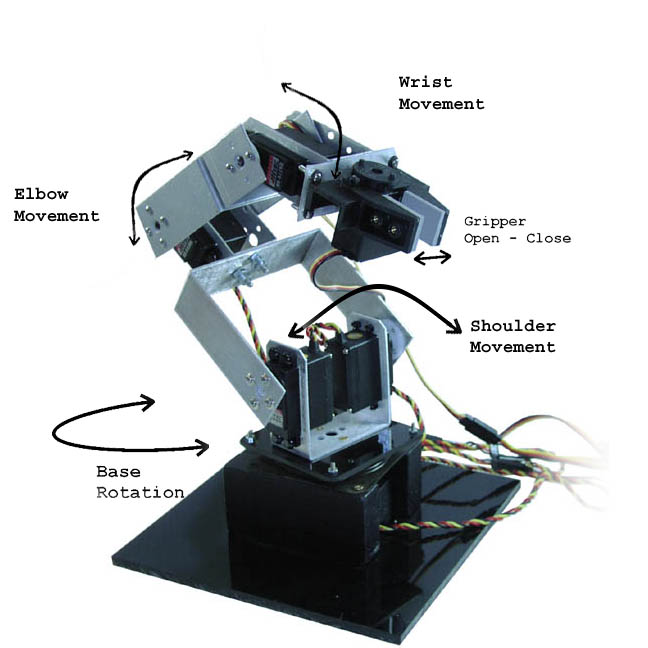
\includegraphics[width=3.5in, height=4.5in]{Figures/Figure1}}
  \end{center}
  \centering
	\parbox{3.5in}{\caption{Robotic arm movement. Source: IMAGESSI, \textbf{\textit{Robotic arm kit}}. Images Scientific Instruments,
http://www.imagesco.com/kits/robotic-arm.html, accessed Aug. 2012, n.d.} \label{fig1}} 
\end{figure}

\subsection{Manufacturing and Product Design}

Computer-aided design (CAD), also known as computer-aided design and drafting (CADD), \cite{CAD} is the use of computer systems to assist in the creation, modification, analysis, or optimization of a design \cite{CAD1}. In simple terms, it means the design of products using computer technology before they are actually manufactured. These products can be of any type, including Lego blocks, automobile machinery, furniture, spare parts, dyes etc. Since these are real world objects, computational geometry obviously plays a major role in the design of these products, their alignment with respect to each other, their shape and how each part would fit into each other. Computer-aided manufacturing (CAM) is the use of computer software to control machine tools and related machinery in the manufacturing of workpieces \cite{CAM3, CAM2, CAM4, CAM5, CAM1}. In short it involves the actual manufacturing of the design or prototype built using CAD packages. CAM also involves many challenges for geometric algorithms, especially assembly decisions and testing of the manufactured product. 

\subsection{Molecular Biology}

Molecular Biology has a high demand for geometry algorithms to model and analyze large scale molecular models associated with proteins, DNA, etc.  The human genome project is producing more-and-more data every day, and using it to produce and investigate models of the basis of life and evolution is an enormous challenge.  Even at the rudimentary level of cellular mechanisms, breakthroughs in geometric modeling and understanding may be the key to finding cures for genetic diseases.  A specific promising problem is to model the spatial structure of proteins, and use this to design drugs that geometrically bind with their receptors \cite{SOFTSURFER}.

In this research thesis, geometric algorithms are considered primarily in the context of GIS applications. This focus of my research comes in part because I have a few years of experience working in the GIS field. A geographic information science (GIS) integrates hardware, software, and data for capturing, managing, and displaying all forms of geographically referenced information. GIS allow us to view, understand, question, interpret, and visualize data in many ways that reveal relationships, patterns, and trends in the form of maps, globes, reports, and charts. A GIS helps you answer questions and solve problems by looking at your data in a way that is quickly understood and easily shared \cite{esriDef}. Answering these geographic questions is not a trivial task and often requires detailed understanding of the algorithms required to solve these problems. Geometric algorithms are heavily used in this area and are typically included as a geo-processing tool in most of the GIS software.

To give a simple example, consider that Starbucks coffee chain wants to open a new store in the state of California. The company will want to determine the optimum location as a function of numerous variables characterizing the available physical space and the socioeconomic demographics around it. This process, if done manually by a person with expertise, can literally take many days and even weeks to produce a correct answer. This task can be completed in a few minutes with the help of the right geo-processing tools, which internally implement computational geometric algorithms (for example the Voronoi diagram). Some of the variables this tool would take into consideration are the population density, average income, proximity of existing stores, other competing stores, etc. These algorithms must be made as efficient as possible because they typically operate on huge datasets and do many complex calculations for each item.

These are some of the areas in which geometry algorithms play a critical role.  Since everything we see and touch has a geometric aspect enabling us to understand our world, and the computer graphics and geometry ball is on the roll and gaining momentum, more-and-more areas of endeavor will start to be influenced by geometry algorithms.  You will recognize them when you see them.  But, will you know the best algorithms for new areas of application?  Knowing the fundamentals, and the scope of our current knowledge will help.

% Note that if you want something in single space you can go back and
% forth between single space and normal space by the use of \ssp and
% \nsp.  If you want doublespacing you can use \dsp.  \nsp is normally
% 1.5 spacing unless you use the doublespace option (or savepaper
% option)
%
%(FORMAT) usually you *don't* want to mess with the spacing for your
%(FORMAT) final version.  If you think/know that the thesis template
%(FORMAT) and/or thesis style file is incorrect/incomplete, PLEASE
%(FORMAT) contact the maintainer.  THANK YOU!!!

\chapter{BACKGROUND}
\label{chap:intro}
% By labeling the chapter, I can refer to it later using the
% label. (\ref{chap:background}, \pageref{chap:background}) Latex will take care
% of the numbering.

In this research thesis, geometric algorithms are considered primarily in the context of GIS applications. This focus of my research comes in part because I have a few years of experience working in the GIS field. A geographic information science (GIS) integrates hardware, software, and data for capturing, managing, and displaying all forms of geographically referenced information. GIS allow us to view, understand, question, interpret, and visualize data in many ways that reveal relationships, patterns, and trends in the form of maps, globes, reports, and charts. A GIS helps you answer questions and solve problems by looking at your data in a way that is quickly understood and easily shared \cite{esriDef}. Answering these geographic questions is not a trivial task and often requires detailed understanding of the algorithms required to solve these problems. Geometric algorithms are heavily used in this area and are typically included as a geo-processing tool in most of the GIS software.

To give a simple example, consider that Starbucks coffee chain wants to open a new store in the state of California. The company will want to determine the optimum location as a function of numerous variables characterizing the available physical space and the socioeconomic demographics around it. This process, if done manually by a person with expertise, can literally take many days and even weeks to produce a correct answer. This task can be completed in a few minutes with the help of the right geo-processing tools, which internally implement computational geometric algorithms (for example the Voronoi diagram). Some of the variables this tool would take into consideration are the population density, average income, proximity of existing stores, other competing stores, etc. These algorithms must be made as efficient as possible because they typically operate on huge datasets and do many complex calculations for each item.

These are some of the areas in which geometry algorithms play a critical role.  Since everything we see and touch has a geometric aspect enabling us to understand our world, and the computer graphics and geometry ball is on the roll and gaining momentum, more-and-more areas of endeavor will start to be influenced by geometry algorithms.  You will recognize them when you see them.  But, will you know the best algorithms for new areas of application?  Knowing the fundamentals, and the scope of our current knowledge will help.

\section{Algorithms}

The past three decades have seen phenomenal advances in our knowledge about geometry algorithms.  The activity has been so great and so original that one might even consider it to be a long overdue revival.  It is more than just shaking the bones of Greek skeletons in front of us.  The massive nature of the problems involved goes as far beyond the Greeks as they went beyond the Egyptians \cite{SOFTSURFER}.  Some of the most significant achievements are given in a recent (1996) report ``Strategic Directions in Computational Geometry" \cite{STRATEGICDIRCG}. Other notable examples are:

\subsection{Voronoi Diagram}

The partitioning of a plane with n points into convex polygons such that each polygon contains exactly one generating point and every point in a given polygon is closer to its generating point than to any other is known as a Voronoi diagram \cite{Voronoi}. Lots of useful information can be gathered from the Voronoi diagram. For example, if the polygons have common boundary then the sites located in these polygons are likely to be in direct competition for customers which live in those regions. Hot spots where the distance between the sites and the people are greater than a minimum threshold can be easily figured out which can be potential places for new stores to be setup. These types of information can be a lot of help in taking strategic business decisions. Besides these there are other useful applications of the Voronoi diagram. 
\begin{itemize}
\item In mining, Voronoi polygons are used to estimate the reserves of valuable materials, minerals or other resources. Exploratory drill holes are used as the set of points in the Voronoi polygons.
\item In machine learning, Voronoi diagrams are used to do 1-NN classifications \cite{MachineLearning}.
\item Voronoi diagrams are also used to compute the roundness of a set of points.
\end{itemize}

Consider another example where a highly flammable liquid needs to be transported by road from location A to location B. The driver would certainly not use the normal geographical positioning system (GPS) which we use in our cars to find the route. In this special scenario the driver does not care about the shortest route in order to save the gas cost. The driver would try to avoid densely populated city areas and roads with steep slopes. These geographic factors need to be considered so that in case of any accident or spills there would be least casualty and harm to common people. Again a Voronoi diagram could be used, but with a different and likely non-uniform distance metric. Still, other geometric algorithms may be used, depending on the choices made by the software developer about representation of relevant information and so on. Solving this can be done in a few minutes or possibly even seconds using a good geo-processing tool. Such a tool can use existing files about geographic information from the area to help the developer even decide on those representation issues and other constraints that permit the modeling of this problem.

\subsection{Polygon Triangulation}

Triangulation or Polygon Triangulation is a fundamental problem in computational geometry, because the first step in working with complicated geometric objects is to break them into simple geometric objects. The simplest geometric objects in a two dimensional space is a triangle. Classical applications of triangulation include finite element analysis and computer graphics. A particularly interesting application of triangulation is surface or function interpolation. Suppose that we have sampled the height of a mountain at a certain number of points. How can we estimate the height at any point (Q) in the plane? If we project the points on the plane, and then triangulate them, the triangulation completely partitions the plane into regions. We can estimate the height of Q by interpolating among the three points of the triangle that contains it. Further, this triangulation and the associated height values define a surface of the mountain suitable for graphics rendering. 

Another important and useful application is to strategically place security cameras in order to guard a restricted place. These cameras are usually hung from the ceiling and it is important to place the cameras at strategic locations so that it covers all the regions and at the same time have minimum number of cameras in order to minimize the cost. This problem can be easily solved using polygon triangulation algorithm. A camera position in the gallery corresponds to a point in the polygon. A camera sees those points in the polygon to which it can be connected with an open segment that lies in the interior of the polygon.

\subsection{Point Location}

Point Location is another hot topic and algorithm which is now-a-days famous. This algorithm basically tries to find the location of point in the space. In simple terms this means to find the query point in a plane which could be comprised of several disjoint regions. Point location queries arise in various settings. The simplest and most common example is to find the current location while driving a car using a global positioning system (GPS). Another application in terms of computer systems is to find the region where the user clicked using the mouse button. The task here is to find the region on the screen where the user clicked the mouse button which could be a button, image, list box or simply nothing but desktop.

\subsection{Delaunay Triangulation}

A Delaunay Triangulation for a set P of points in a plane is a triangulation DT(P) such that no point in P is inside the circumcircle of any triangle in DT(P). Delaunay triangulations maximize the minimum angle of all the angles of the triangles in the triangulation; they tend to avoid skinny triangles. The triangulation is named after Boris Delaunay for his work on this topic from 1934. \cite{Delanuay, SOFTSURFER, DelanuayWiki}
\begin{itemize}
\item The Euclidean minimum spanning tree \cite{SpannigTree} of a set of points is a subset of the Delaunay triangulation of the same points, and this can be exploited to compute it efficiently. 
\item For modeling terrain or other objects given a set of sample points, the Delaunay triangulation gives a nice set of triangles to use as polygons in the model. In particular, the Delaunay triangulation avoids narrow triangles (as they have large circumcircles compared to their area).
\item Delaunay triangulations can be used to determine the density or intensity of points samplings by means of the DTFE. \cite{DTFE}
\item Delaunay triangulations are often used to build meshes for space-discretized solvers such as the finite element method and the finite volume method of physics simulation, because of the angle guarantee and because fast triangulation algorithms have been developed. Typically, the domain to be meshed is specified as a coarse simplified complex; for the mesh to be numerically stable, it must be refined, for instance by using Ruppert's algorithm. \cite{RuppertAlgo}
\end{itemize}

\section{Maps and Geographic Information Science (GIS)}

Maps are an invaluable source of information and are used in many day to day activities. Maps have been used since olden days, although maps in those days were not accurate and not scaled properly. But since the last century, mankind has realized the importance of maps and learned proper means of creating and using them; today�s maps are often derived from very precise satellite information. If a map is not constructed properly then it can definitely be a source of frustration. But now-a-days maps are really easy to understand and interpret. Thanks to the vast area of study in geography and evolution of new technology. In today�s world we have digital maps that are really easy to interact with and reveal a wealth of information. A geographic information system splits maps into several layers that are super imposed upon each other and thus present a map that is really a stack of layers drawn on top of one another. For example, consider a map showing the vegetation in the state of California. Initially there would be a layer drawing the map of the state of California and then there would be second layer showing the vegetation that would be drawn on top of the layer of California. The first layer is usually called as a Basemap Layer. It is very important that all the layers in map are in sync with each other.  In GIS terms this is referred to as a spatial reference. Spatial reference is the coordinate system, tolerance, and resolution used to store the spatial dataset. In other words consider spatial reference as the reference point with respect to with, each layer is drawn. In a digital map the visibility of any layer can be turned off easily by the click of a mouse button thus giving the user the power to hide/ unhide any information at any particular instance of time. 

Having given some preliminary description about computational geometry, its algorithms, geographic information science (GIS) and maps we will now turn our attention to the contribution of this thesis research.  This thesis research is about a particular type of spatial algorithm which is commonly known as a Line Sweep Algorithm or Plane Sweep Algorithm. There are many algorithms that use the line-sweep technique. One algorithm in particular tries to find intersections among line segments belonging to two different sets in a two dimensional co-ordinate system. The problem of finding and reporting all pair-wise intersections in a set of line segments is among the first to have been studied in computational geometry; its solution established the use of sweep-line methods and introduced the notion of output sensitive algorithms. In the early days of computational geometry, Bentley and Ottmann \cite{BentleyOttmann} introduced their well-known line sweep algorithm. Mairson and Stol \cite{Stol} were the first to find an asymptotically optimal algorithm running in {\it O}(n log n + k) time.

Consider that a city planner wants to find out the location where there is a need to build bridges. The city planner would first prepare a map of the city. This data is generally freely available on most government and educational websites. Then the planner would put a layer of rivers flowing through the city and finally he/she would put a layer of roads in the city on top of the rivers (Figure.~\ref{fig2} \cite{MAP}). Now the answer to the question of the places where bridges need to be built is basically the places where roads and rivers intersect. The line sweep algorithm can be useful in finding the solution to this question. The rivers are generally not straight and are curvy. These curved lines can be represented by a collection of many small adjacent segments. Then one set of line segments can represent the rivers flowing through the city and the second set of line segments can represent the roads in the city. Now we need to find out intersections among these line segments, which might be appropriate candidates for places where bridges need to be built. This algorithm to find intersections among set of line segments seems trivial. But this is a complex algorithm and must be highly efficient, especially given the potentially large number of segments involved in a real world situation as described. Imagine running this algorithm on tera-bytes of a raster image and finding out the correct result in a matter of few seconds.
\begin{figure}[ht]
  \begin{center}
   	\fbox{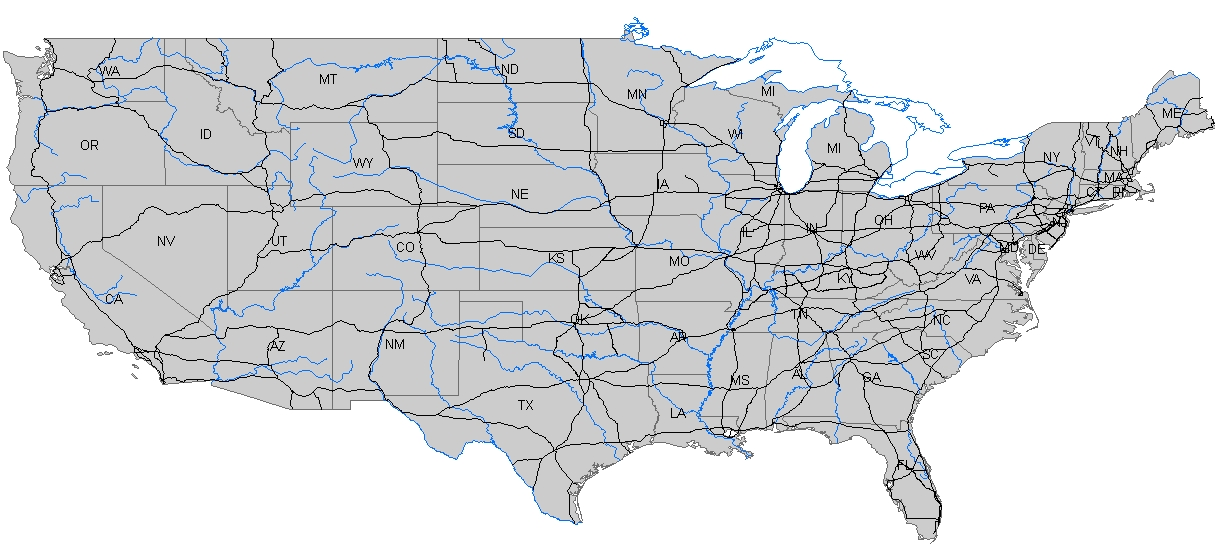
\includegraphics[width=4.5in]{Figures/Figure2}}
  \end{center}
  \centering
	\parbox{4.5in}{\caption{Map of USA showing roads and rivers. Source: ESRI, \textbf{\textit{Arcgis online}}. ArcGIS, http://www.arcgis.com, accessed Aug. 2012, n.d.} \label{fig2}} 
\end{figure}

Other algorithms that typically use the line sweep technique are Voronoi diagrams, finding nearest object, triangulation, two-dimensional and three-dimensional point location, shortest path and many others in GIS as well as in other fields.

I was once asked a question during an interview; it was amazing how easily I could relate the question to this algorithm and present a solution. I was given a scenario where there is a multinational company that has three phone servers. People could make calls at any time during the day. I was asked to propose an algorithm that would determine the peak time during the day when most calls were made. I thought for about 5-10 minutes and suddenly it struck my mind that this problem can be solved using the line sweep algorithm. Imagine a two dimensional space for each server where x-axis is represented by the duration of phone call and y-axis is represented by the time in a day. Then we would get several lines representing the calls made during that day for each server as horizontal lines in the XY co-ordinate space. Now image a horizontal line sweeping this graph from top to bottom. Each time it would intersect the calls made during the day, we would record the total number of intersections intersection. When the imaginary line sweeps the graph completely then we would have the answer for the peak time when maximum calls were made during the day.

Like this example, there are many other scenarios where a line sweep algorithm might be useful, which makes me appreciate this algorithmic technique even more. I studied this algorithm and thought of altering one of the data structure used by it. The goal of the alteration would be to enhance the efficiency of this algorithm by modifying one of the data structure used by line-sweep algorithm, namely status structure such as in the line-segment intersection problem, is the objective of this research. The status structure is used to keep track of the segments currently adjacent to one another and the proposed alteration will increase the efficiency of search operations on this structure.

\section{Supporting Research}
Several other people have worked and been working on various aspect of this algorithm. Many of them have published papers regarding their work. It is quite interesting to see so much work going around in this work on this algorithm. Notable among the published papers are ``Feature Analysis Using Line Sweep Thinning Algorithm" \cite{FeatureAccessThinningAlgo} and ``A Sweep line approach to Interconnect Testing" \cite{InterconnectTesting}.

% Note that if you want something in single space you can go back and
% forth between single space and normal space by the use of \ssp and
% \nsp.  If you want doublespacing you can use \dsp.  \nsp is normally
% 1.5 spacing unless you use the doublespace option (or savepaper
% option)
%
%(FORMAT) usually you *don't* want to mess with the spacing for your
%(FORMAT) final version.  If you think/know that the thesis template
%(FORMAT) and/or thesis style file is incorrect/incomplete, PLEASE
%(FORMAT) contact the maintainer.  THANK YOU!!!

\chapter{LINE SEGMENT INTERSECTION}
\label{chap:linesegintersec}
% By labeling the chapter, I can refer to it later using the
% label. (\ref{chap:linesegintersec}, \pageref{chap:linesegintersec}) Latex will take care
% of the numbering.

\section{Problem Definition}

Consider the example given in the previous chapter to find the intersections between roads and rivers in order to find the locations where bridges need to be built in the city. This problem is commonly known as the map overlay problem where the map of roads and rivers are superimposed upon each other. Roads and rivers are represented by lines and we need to find the intersection points among those lines or the region induced by those line intersections. We are going to consider an efficiency-minded modification of the algorithm for the simple case of finding the intersection points among line segments as the scope of this thesis. Let�s describe the problem geometrically first. Consider the rivers as one set of line segments and roads as another set of segments. We then need to find the point of intersection between these two sets of segments. However, the problem specification is not yet precise enough. We have not specified what to do in various degenerate cases, such as when two line segments intersect because their endpoints meet at a common point.  We could require two line segments always to intersect only in the interior of the lines.  This essentially becomes the question of whether the two line segments are open or closed. As with the representation of curved features in a map, we will make some assumptions that simplify the approach. Later we shall realize that it is easy to consider these special cases without changing the basic nature of the algorithm. We will assume the line segments to be such that they are open (we do not have to worry about endpoint-only intersections--said another way, we will consider the point as an intersection point even if it happens to be on the end of the line segment) and no more than two line segments intersect at a single point (we do not have to worry about multiple intersections in the same place). Furthermore, none of the line segments are parallel to each other. 

For the sake of simplicity and without loss of generality, we will consider the line segments from two different sets (e.g. rivers and roads) to be members of a single set. We will compute the intersection among all the lines in this single set. We will obviously get some intersection points among the same set of line segments when we merge these two sets together, and we can remove this ambiguity later. To do this we simply store the original segments involved so that at the end we can discard the intersection points which belong to segments from the same original set. Thus the required intersection points can be filtered out easily. Storing of these line segments along with the intersection points may seem like a bit of storage overhead at first glance but most of times it is often required in other places too. Let�s say that we want to consider the intersection points among line segments based on the spatial extent. In that case we would need the information about the intersecting line segments in order to filter them out based on the spatial extent. Finally we will state our problem specification as follows: given a set S of n closed segments in the plane (Figure.~\ref{fig3} \cite{TEXTBOOK}), report all intersection points among the segments in S.
\begin{figure}[ht]
  \begin{center}
   	\fbox{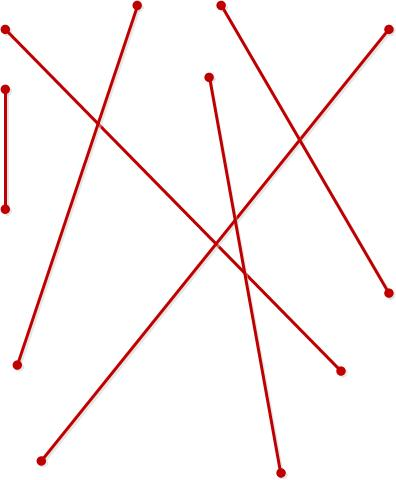
\includegraphics[width=3in, height=2.5in]{Figures/Figure3}}
  \end{center}
  \centering
	\parbox{3in}{\caption{Segments in a 2-dimensional space. Adapted from Source : M. DE BERG, M. VAN KREVELD, M. OVERMARS, AND O. SCHWARZKOPF,
\textbf{\textit{Computational Geometry- Algorithms and Applications}}, Springer Verlag, Berlin, Germany, 2000, ch. 2, pp. 19-29.} \label{fig3}} 
\end{figure}

\section{Potential Solution}

This may seem like an easy problem at first glance where we simply need to take each line segment and perform intersection tests with each of the other line segments. This algorithm would require O(n2) time. Unfortunately this would actually be the optimal solution in the case where all the line segments in a set intersect with every other line segment in the other set. This is called an output-bound problem. We may find an efficient algorithm in general, but certain so-called pathological cases can cause its running time to degenerate into this worst-case quadratic performance. In practical situations, however, most segments intersect none or only a few of the other segments. Thus the total number of intersection points is quite less and seldom leads to this quadratic performance. As we will see, the algorithm is as efficient as possible (that is, it is optimal) except in these rare cases. 

\section{Draft of the Algorithm}

How could we avoid testing all the pairs of line segments for intersection in order to improve the asymptotic time (in the general, non-pathological arrangement)? We can make use of the geometry of the situation and perform intersection tests only of the segments that are close to each other at some point in our algorithm. This is based on the geometric insight that segments must become close to each other to intersect. How do we find out which line segments are close to each other? What do we exactly mean by being close to each other (for example horizontally or vertically or along some other direction)?

Let L := {La, Lb, �, Ln} be the set of segments for which we want to compute all the intersections. Now we need to find out which segments among these are close to each other. Consider the y-interval of these line segments to be its orthogonal projection onto y-axis (Figure.~\ref{fig4} \cite{TEXTBOOK}). Now when the y-interval of two or more segments overlaps then these segments are considered close to each other and we can perform intersection tests on them. The line segments whose y-interval does not overlap are far apart in the y direction and cannot intersect with each other. Thus we only need to test the pair of segments whose y-intervals overlap with each other. In other words, we need to test the pair of segments for which there exists a horizontal line that intersects both the segments, given that no other segments, besides the two in the pair, are intersected by the horizontal line at any point between the intersections between it and the pair. To be more precise about finding these pairs, consider an imaginary line �S� sweeping downwards over the plane starting at a position above all the line segments. We can keep track of the line segments intersecting this sweeping line as it moves downwards.

This algorithmic technique is called the line-sweep (or sometimes plane-sweep) algorithm and the line �S� is called the sweep line. The data structure that maintains information about the set of lines segments intersecting the sweep line at any given point is called the status of the sweep line. This data structure, called the status structure, is typically implemented as a kind of balanced binary search tree. The status changes as the sweep line moves downwards but it does not need to be updated continuously. The status structure is updated only at certain points called event points. These event points are the end points of the line segments, as well as intersection points that are discovered along the way (Figure.~\ref{fig5} \cite{TEXTBOOK}).
\begin{figure}[ht]
  \begin{center}
   	\fbox{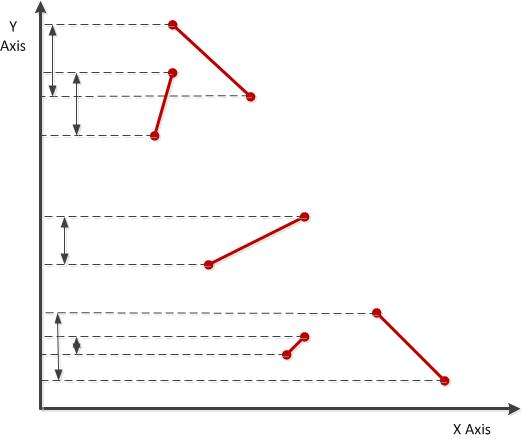
\includegraphics[width=3.5in, height=3.5in]{Figures/Figure4}}
  \end{center}
  \centering
	\parbox{3.5in}{\caption{Lines showing their orthogonal projection onto Y axis. Adapted from Source: M. DE BERG, M. VAN KREVELD, M. OVERMARS, AND O. SCHWARZKOPF, \textbf{\textit{Computational Geometry- Algorithms and Applications}}, Springer Verlag, Berlin, Germany, 2000, ch. 2, pp. 19-29.} \label{fig4}} 
\end{figure}

When the sweep line reaches these end points, it is only then that the status structure is updated and the algorithm actually does something. When the sweep line reaches the upper end point of a line segment, then a new segment starts intersecting the sweep line and intersection test is performed against all the line segments adjacent to each other along the sweep line at that point. If the end point is the lower end point of the line segment then that segments stops intersecting the sweep line and that line segment can be deleted from the status structure (the sweep line will never again encounter it). This is how we only perform the intersection tests on segments that are �close� or  adjacent, i.e. for which the horizontal line passes through them in succession, excluding all other pairs and thereby affording us the avoidance of the quadratic check of every pair and improving the efficiency of the algorithm.
\begin{figure}[ht]
  \begin{center}
   	\fbox{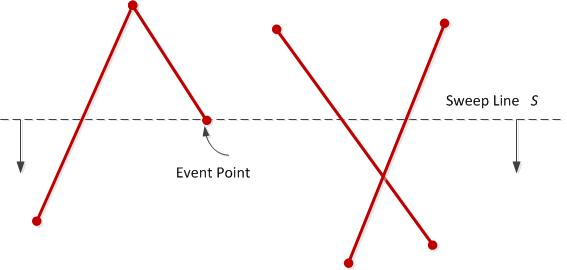
\includegraphics[width=6in, height=3in]{Figures/Figure5}}
  \end{center}
  \centering
	\parbox{6in}{\caption{Event point of a line. Adapted from Source: M. DE BERG, M. VAN KREVELD, M. OVERMARS, AND O. SCHWARZKOPF, \textbf{\textit{Computational Geometry- Algorithms and Applications}}, Springer Verlag, Berlin, Germany, 2000, ch. 2, pp. 19-29.} \label{fig5}} 
\end{figure}

\section{Some Problems and their Solutions}

Unfortunately this approach can fail in certain conditions. We can still end up performing intersection tests on a quadratic number of pairs even though there may actually be substantially fewer intersections. A simple example can be where we have a number of vertical lines that intersect x-axis. The problem is that the two segments that intersect the sweep line can still be far apart in the horizontal direction even though they are closer in the y direction.

To solve this problem, let us order the line segments from left to right. Now we will perform intersection tests only on the segments that are adjacent to each other so that we test only the segments that close to each other in the horizontal direction. Thus each line segment is tested for intersection with two adjacent line segments, namely, one to left and other to the right of it. This comparison is made based on the upper end point. The status should now correspond to this new strategy reflecting the ordered sequence of segments intersecting the sweep line. Thus the new status now not only changes at the end points of the line segments but it also changes at the intersection points which are computed at runtime on the fly. When a sweep line intersects an intersection point (Figure.~\ref{fig6} \cite{TEXTBOOK}), we must test the two segments for intersection against their new neighbors. This is a new type of event point besides the regular upper and lower end points of line segments.
\begin{figure}[ht]
  \begin{center}
   	\fbox{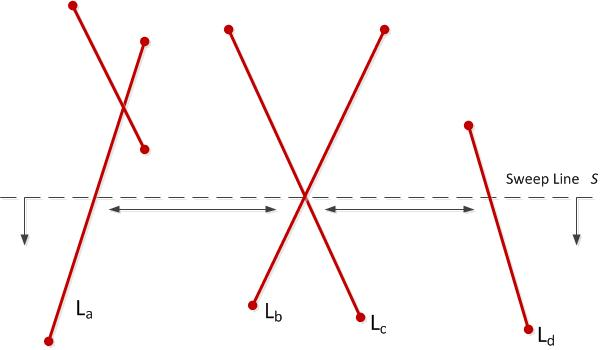
\includegraphics[width=5in, height=1.75in]{Figures/Figure6}}
  \end{center}
  \centering
	\parbox{5in}{\caption{Lines have new neighbors. Adapted from Source: M. DE BERG, M. VAN KREVELD, M. OVERMARS, AND O. SCHWARZKOPF, \textbf{\textit{Computational Geometry- Algorithms and Applications}}, Springer Verlag, Berlin, Germany, 2000, ch. 2, pp. 19-29.} \label{fig6}} 
\end{figure}

Let�s discuss the approach we have discussed until now. Imagine there are n number of line segments in a two dimensional space. Now imagine a sweep line �S� that starts sweeping all the line segments. Initially the sweep line is placed above all the line segments. The sweep line maintains a status structure that indicates all the ordered line segments from left to right that intersect the sweep line at any particular instance of time. This status structure is updated at certain points called as event points. These event points are namely upper end point of a line segment, lower end point of a line segment and the intersection point of line segments that are detected at runtime (Figure.~\ref{fig8} \cite{TEXTBOOK}). We have to take several actions depending upon the type of event point.
\begin{figure}[ht]
  \begin{center}
   	\fbox{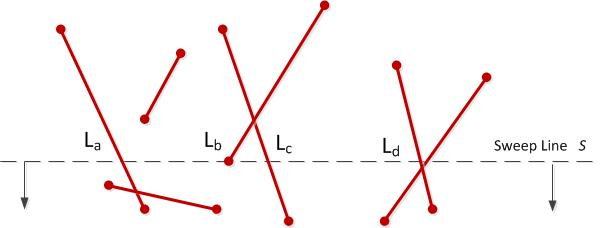
\includegraphics[width=5in, height=2in]{Figures/Figure8}}
  \end{center}
  \centering
	\parbox{5in}{\caption{Sweep line progressing through lines. Adapted from Source: M. DE BERG, M. VAN KREVELD, M. OVERMARS, AND O. SCHWARZKOPF, \textbf{\textit{Computational Geometry- Algorithms and Applications}}, Springer Verlag, Berlin, Germany, 2000, ch. 2, pp. 19-29.} \label{fig8}} 
\end{figure}

When the event point is an upper end point of a line segment then the sweep line starts intersecting a new line segment. This line segment must be inserted at appropriate position in the status structure and an intersection test must be performed against its two neighbors namely one to left and the other to the right side of it. When the event point is a lower end point of a line segment then the sweep line has reached the bottom of that line segment and hence will stop intersecting it. It must be deleted from the status structure and its neighbors must be considered for intersection as they now become new neighbors of each other. 

When the event point is an intersection point (Figure.~\ref{fig9} \cite{TEXTBOOK}) the two segments that intersect each other change their order along the sweep line. Each of them gets (at most) one new neighbor, against which they are tested for intersection. At each event point only the intersection point found below the sweep line are taken into consideration since those that are above the sweep line have already been detected and processed (Figure.~\ref{fig7} \cite{TEXTBOOK}). When all the event points are processed, then algorithm indicates that we have swept the plane all the way to the bottom and detected all the event points.
\begin{figure}[ht]
  \begin{center}
   	\fbox{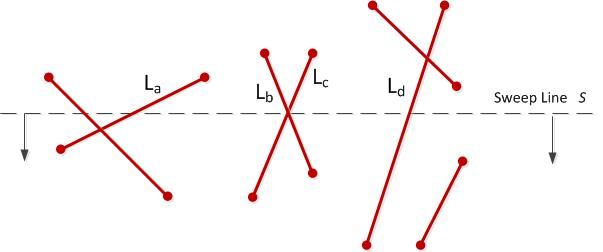
\includegraphics[width=6in, height=3in]{Figures/Figure9}}
  \end{center}
  \centering
	\parbox{6in}{\caption{Sweep line reaching an intersection point. Adapted from Source: M. DE BERG, M. VAN KREVELD, M. OVERMARS, AND O. SCHWARZKOPF, \textbf{\textit{Computational Geometry- Algorithms and Applications}}, Springer Verlag, Berlin, Germany, 2000, ch. 2, pp. 19-29.} \label{fig9}} 
\end{figure}
\begin{figure}[ht]
  \begin{center}
   	\fbox{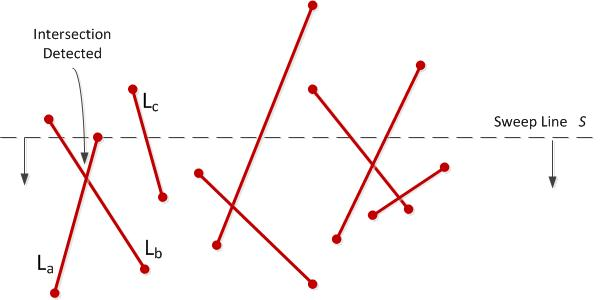
\includegraphics[width=6in, height=3in]{Figures/Figure7}}
  \end{center}
  \centering
	\parbox{6in}{\caption{Snapshot when an intersection point is detected. Adapted from Source: M. DE BERG, M. VAN KREVELD, M. OVERMARS, AND O. SCHWARZKOPF, \textbf{\textit{Computational Geometry- Algorithms and Applications}}, Springer Verlag, Berlin, Germany, 2000, ch. 2, pp. 19-29.} \label{fig7}} 
\end{figure}

% Note that if you want something in single space you can go back and
% forth between single space and normal space by the use of \ssp and
% \nsp.  If you want doublespacing you can use \dsp.  \nsp is normally
% 1.5 spacing unless you use the doublespace option (or savepaper
% option)
%
%(FORMAT) usually you *don't* want to mess with the spacing for your
%(FORMAT) final version.  If you think/know that the thesis template
%(FORMAT) and/or thesis style file is incorrect/incomplete, PLEASE
%(FORMAT) contact the maintainer.  THANK YOU!!!

\chapter{THE ALGORITHM}
\label{chap:thealgorithm}
% By labeling the chapter, I can refer to it later using the
% label. (\ref{chap:thealgorithm}, \pageref{chap:thealgorithm}) Latex will take care
% of the numbering.

In this chapter we will take a look at the details of the algorithm that we have been talking in the previous chapters. This is the algorithm which finds out the actual intersection points among a set of line segments in a two dimensional space. Though this algorithm is primarily for a two dimensional space.  It can be easily extended for 3 or n dimensional space with slight modification. Right now we will be limiting ourselves to 2 dimensional primary version of the algorithm.

\section{Data structures}

The algorithm requires several data structures. The first one is called as the event queue which stores all the events. We will denote the event queue by `Q'. The data structure that represents the `Q' should basically support the operations for fetching (removing) the next event so that it can be processed. This next event that needs to be fetched should be the highest event point below the sweep line. So the event points should be stored efficiently such that the events are fetched in right order with least time. If two event points are on the same horizontal line then the left event point is returned first. So imagine that the horizontal sweep line in inclined a bit downwards on the left side (Figure.~\ref{fig10} \cite{TEXTBOOK}) so that it reaches the left event points first than the right event points falling on the same horizontal line. 
\begin{figure}[ht]
  \begin{center}
   	\fbox{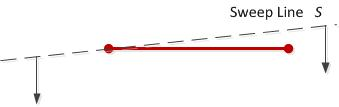
\includegraphics[width=4in, height=1.5in]{Figures/Figure10}}
  \end{center}
  \centering
	\parbox{4in}{\caption{Sweep line passing through a horizontal line. Adapted from Source: M. DE BERG, M. VAN KREVELD, M. OVERMARS, AND O. SCHWARZKOPF, \textbf{\textit{Computational Geometry- Algorithms and Applications}}, Springer Verlag, Berlin, Germany, 2000, ch. 2, pp. 19-29.} \label{fig10}} 
\end{figure}

This data structure should also support the insertion operation because there are some event points like the intersection points, which are computed dynamically, and which needs to be inserted into the event queue. Also many times it may happen that the two event points coincide such that the end points of two event points are the same. In such case we assume that the event point is the same. So the event queue should also support operation to tell if the event point already exists in the queue. It is important to remember that the event queue `Q' should support all these operations while maintaining the integrity of the queue. To summarize the event queue `Q' should support the below operations.
\begin{enumerate}
	\item Insertion
	\item Deletion
	\item Detecting if an event point already exists in the queue.
\end{enumerate}

\section{Implementation}

We will implement the event queue as an AVL tree (Figure.~\ref{fig11} \cite{TEXTBOOK}). We decided not to use heap data structure to implement the queue as this data structure also needs to support the operation of finding whether a given event point is already present in the `Q' which is not possible in the heap. We will define an order a on the event points that represents the order in which they will be handled. Thus if A and B are two event points then we have $A \alpha B$ if and only if A$_y$ $>$ B$_y$ holds or A$_y$ $=$ B$_y$ and A$_x$ $<$ B$_x$ holds. With each event point M we will store the segments whose starting end point is M.
\begin{figure}[ht]
  \begin{center}
   	\fbox{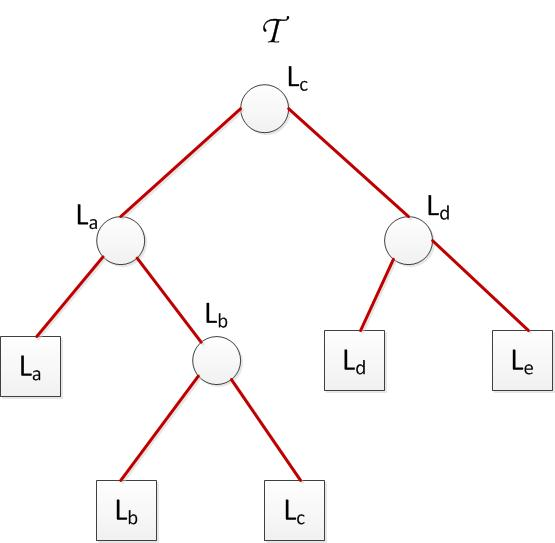
\includegraphics[width=4.5in, height=2.25in]{Figures/Figure11}}
  \end{center}
  \centering
	\parbox{4.5in}{\caption{An AVL tree representing a status structure. Adapted from Source: M. DE BERG, M. VAN KREVELD, M. OVERMARS, AND O. SCHWARZKOPF, \textbf{\textit{Computational Geometry- Algorithms and Applications}}, Springer Verlag, Berlin, Germany, 2000, ch. 2, pp. 19-29.} \label{fig11}} 
\end{figure}	

\section{Status Structure $\tau$}

Second, we need to maintain the status of the algorithm. This data structure is used to maintain the status of lines intersecting the sweep line in an ordered sequence. This data structure is denoted by `$\tau$'. The status structure is used to determine the neighbors of a given segment so that they can be tested for intersection. This status structure must be dynamic as segments continuously start or stop to intersect the sweep line and thus the data structure needs to be maintained accordingly at real time. Whenever a line segments `L' starts to intersect the sweep line `S' it is inserted into `$\tau$' and whenever the line segment stops intersecting `S' then it is deleted from `$\tau$'. The line segment must be inserted at appropriate position into `$\tau$' since it will used to determine the intersection tests with the neighbors. We will use an AVL tree to implement the status structure `$\tau$' (Figure.~\ref{fig12} \cite{TEXTBOOK}).
\begin{figure}[ht]
  \begin{center}
   	\fbox{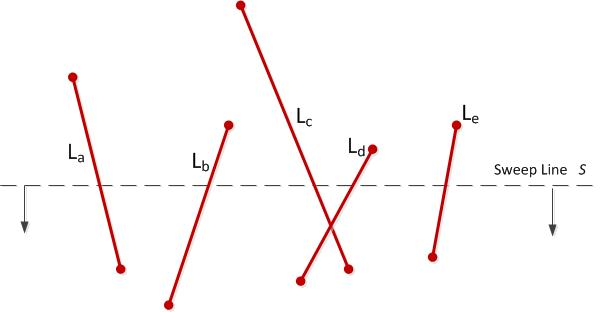
\includegraphics[width=6in, height=3in]{Figures/Figure12}}
  \end{center}
  \centering
	\parbox{6in}{\caption{Actual lines represented by a status structure. Adapted from Source: M. DE BERG, M. VAN KREVELD, M. OVERMARS, AND O. SCHWARZKOPF, \textbf{\textit{Computational Geometry- Algorithms and Applications}}, Springer Verlag, Berlin, Germany, 2000, ch. 2, pp. 19-29.} \label{fig12}} 
\end{figure}

Thus we store the segments intersecting the sweep line ordered in the leaves of the AVL tree `$\tau$'. The left-to-right order of the segments along the sweep line corresponds to the left-to-right order of the leaves in `$\tau$'. At each internal node we must store some data that will guide the search down to the leaves of the tree. At each internal node we store the rightmost segment in the left subtree. Storing of the line segments at the leaf node may sound like some redundant information as this could also be achieved by storing it only in the internal nodes. But it is conceptually simpler to think that the internal nodes should not store the data but only values to guide the search. Also storing of the segments at the leaf node makes the data structure more simple and easy to understand visually. Suppose we search in `$\tau$' for some segment immediately to the right of some point `P' that lies on the sweep line. At each internal node `V' we simply test whether `P' lies to the left of right of the segment stored at `V' and we navigate to the left or right depending on the result, eventually ending up in a leaf node. Either this leaf or the leaf immediately to the right of it is the segment that we are searching for. Similarly we can store the segment immediately to the left of `P' or the segment containing `P'. Thus each update and neighbor search operation takes {/it O}(log n) time. Please note this time complexity as further we will introduce some changes to the data structure `$\tau$' such that it will reduce this time.

\section{Formal Algorithm}

The formal algorithm as stated in the text book [14] is as follows-
\noindent
Algorithm FindIntersections(L) \newline
{\it Input:} A set S of line segments in the plane \newline
{\it Output:} The set of intersection points among the segments in L, with for each intersection point the segments that contain it.
\begin{enumerate}
	\item Initialize an empty queue Q. Next, insert the segment endpoints into Q; when an upper endpoint is inserted, the corresponding segment should be stored with it.
	\item Initialize an empty status structure $\tau$.
	\item while Q is not empty
	\item \hspace*{2em} do Determine the next event point P in Q and delete it.
	\item \hspace*{4em} HandleEventPoint(P)
\end{enumerate}

We have already seen how events are handled: at endpoints of segments we have to insert or delete segments from the status structure $\tau$, and at intersection points we have to change the order of two segments. In both cases we also have to do intersection tests between segments that become neighbors after the event (Figure.~\ref{fig131} \cite{TEXTBOOK}). In degenerate cases, where several segments are involved in one event point, the details are a little bit tricky. The next procedure describes how to handle event points correctly.

\noindent
HandleEventPoint(P)
\begin{enumerate}
	\item Let {\it U}(P) be he set of segments whose upper endpoint is P; these segments are stored with the event point P. (For horizontal segments, the upper endpoint is by definition the left endpoint.)
	\item Find all segments stored in $\tau$ that contain P; they are adjacent in $\tau$ (Figure.~\ref{fig132} \cite{TEXTBOOK}). Let L(P) denote the subset of segments found whose lower endpoint is P, and let C(P) denote the subset of segments found that contain P in their interior.
	\item if L(P) U {\it U}(P) U C(P) contains more than one segment
	\item \hspace*{2em} then Report P as an intersection, together with L(P), U(P), and C(P)
	\item Delete the segments in L(P) U C(P) from $\tau$.
	\item Insert the segments in {\it U}(P) U C(P) into $\tau$. The order of the segments in $\tau$ should correspond to the order in which they are intersected by a sweep line just below P. If there is a horizontal segment, it comes last among all segments including P.
	\item (* Deleting ad re-inserting the segments of C(P) reverses their order. *)
	\item if {\it U}(P) U C(P) = $\phi$
	\item then Let S$_l$ and S$_r$ be the left and right neighbors of P in $\tau$.
	\item \hspace*{2em} FindNewEvent(S$_l$, S$_r$, P)
	\item else Let S` be the leftmost segment of U(P) U C(P) in $\tau$
	\item \hspace*{2em} Let S$_l$ be the left neighbor of S` in $\tau$
	\item \hspace*{2em} FindNewEvent(S$_l$, S`, P)
	\item \hspace*{2em} Let S'' be the rightmost segment of U(P) U C(P) in $\tau$
	\item \hspace*{2em} Let S$_r$ be the rightmost neighbor of S'' in $\tau$
	\item \hspace*{2em} FindNewEvent(S'', S$_r$, P)
\end{enumerate}
\begin{figure}[ht]
  \begin{center}
   	\fbox{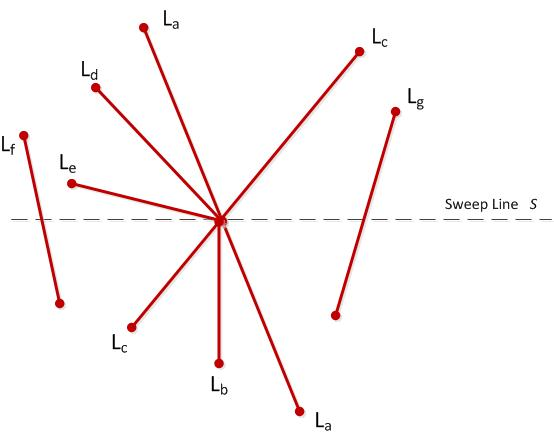
\includegraphics[width=4in, height=2in]{Figures/Figure13-1.jpg}}
  \end{center}
  \centering
	\parbox{4in}{\caption{A snapshot of an instance of sweep line in a running algorithm. Adapted from Source: M. DE BERG, M. VAN KREVELD, M. OVERMARS, AND O. SCHWARZKOPF, \textbf{\textit{Computational Geometry- Algorithms and Applications}}, Springer Verlag, Berlin, Germany, 2000, ch. 2, pp. 19-29.} \label{fig131}} 
\end{figure}
\begin{figure}[ht]
  \begin{center}
   	\fbox{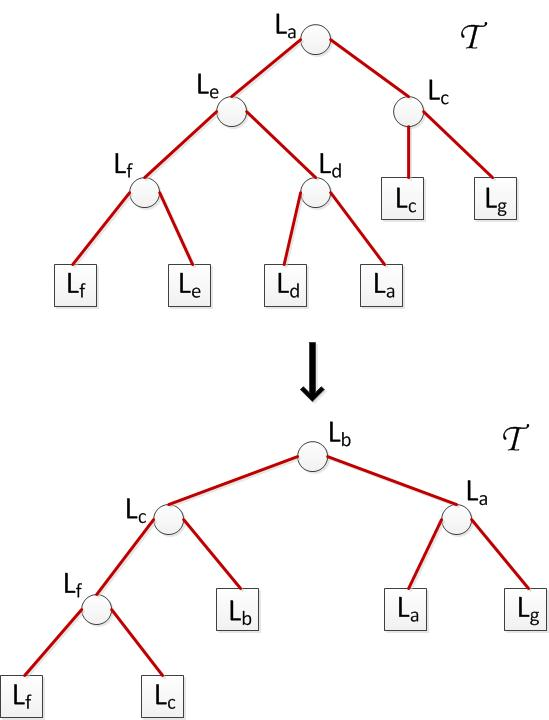
\includegraphics[width=4in, height=4.5in]{Figures/Figure13-2.jpg}}
  \end{center}
  \centering
	\parbox{4in}{\caption{A snapshot of a status structure in a running algorithm. Adapted from Source: M. DE BERG, M. VAN KREVELD, M. OVERMARS, AND O. SCHWARZKOPF, \textbf{\textit{Computational Geometry- Algorithms and Applications}}, Springer Verlag, Berlin, Germany, 2000, ch. 2, pp. 19-29.} \label{fig132}} 
\end{figure}

Note that in lines 8-16 we assume that Sl and Sr actually exists. If they do not exist the corresponding steps should obviously not be performed. The procedures for finding the new intersections are easy: they simply test two segments for intersection. The only thing we need to be careful about is, when we find an intersection, whether this intersection had already been handled earlier or not. When there are no horizontal segments, then the intersection has not been handled yet when the intersection point lies below the sweep line. But how should we deal with horizontal segments? Recall our convention that events with the same y- coordinate are treated from left to right. This implies that we are still interested in intersection points lying left to right of the current event point. Hence the procedure FindNewEvent is defined as follows.

\noindent
FindNewEvent(S$_l$, S$_r$, P)
\begin{enumerate}
	\item if S$_l$ and S$_r$ intersect below the sweep line, or on it and to the right of the current event point P, and the intersection is not yet present as an event in Q.
	\item \hspace*{2em} then Insert the intersection point as an event into Q.
\end{enumerate}
	
The algorithm that we just presented is output sensitive algorithm. This is a very important point as the algorithm time complexity depends not only on the input to the algorithm but it also depends on the output. In our case the output is the total number of intersection points. The pseudo code of the implemented algorithm is provided in Appendix~B.

\section{Time Complexity}

The total running time of the algorithm is {\it O}(( n + m ) log n) where n is the input size and m is the total number of intersection points. One intersection point can consists of a large number of segments, namely in the case where many segments intersect in a common point.

At the very beginning of the algorithm the event queue Q is constructed which takes {\it O}(n log n) time because we decided to implement the event queue as an AVL tree. The status structure initialization takes constant time. Then the algorithm starts out to handle each event point. There could be at the most three operations performed on each event
\begin{enumerate}
	\item The event itself is deleted from the event queue �Q� in step 5 of the algorithm. This will take {\it O}(log n) time each.
	\item There can be one or two calls to FindNewEvent which may cause at most two new events to be added to the event queue. This would also take {\it O}(log n) time each.
\end{enumerate}

We also perform the operations of inserting, deletion and finding neighbor on the status structure �$\tau$� that should take {\it O}(log n) time each. These number of operations are linear in the number m(p) := card(L(p) U  {\it U}(p) U  c(p)), over all event points p, by m, the running time of the algorithm is {\it O}(m log n). It is clear that m = {\it O}(n + k) where k is the output which is the total number of intersection points \cite{TEXTBOOK}. Also please note that the insertion, deletion and finding nearest neighbor in an AVL tree taken {\it O}(log n) time. The contribution of this research is to optimize the time required to compute the nearest neighbor which is one of the most frequent operation performed by the algorithm.

% Note that if you want something in single space you can go back and
% forth between single space and normal space by the use of \ssp and
% \nsp.  If you want doublespacing you can use \dsp.  \nsp is normally
% 1.5 spacing unless you use the doublespace option (or savepaper
% option)
%
%(FORMAT) Usually you *don't* want to mess with the spacing for your
%(FORMAT) final version.  If you think/know that the thesis template
%(FORMAT) and/or thesis style file is incorrect/incomplete, PLEASE
%(FORMAT) contact the maintainer.  THANK YOU!!!

\chapter{BINARY SEARCH TREES}
\label{chap:binarysearchtree}
% By labeling the chapter, I can refer to it later using the
% label. (\ref{chap:binarysearchtree}, \pageref{chap:binarysearchtree}) Latex will take care
% of the numbering.

The single most heavily used data structure in line sweep algorithm is binary search tree (BST), hence it is worth to spend an entirely dedicated chapter to explain this data structure and how it is used in this algorithm. Although the algorithm uses slightly modified binary search tree but still the main concept is that of a binary search tree. In fact the algorithm uses an AVL tree. Hence it is imperative to understand this data structure in order to properly understand the working of the algorithm.

\section{Definition and Properties}

In computer science, a binary search tree (BST), which may sometimes also be called an ordered or sorted binary tree, is a node-based binary tree data structure which has the following properties \cite{BSTWIKI}:
\begin{itemize}
	\item The left subtree of a node contains only nodes with keys less than or equal to the node's key.
	\item The right subtree of a node contains only nodes with keys greater than the node's key.
	\item Both the left and right subtrees must also be binary search trees.
\end{itemize}

Since each node in a binary search tree has only two child nodes and hence the name binary search tree. The only exception to the nodes having two child nodes is the bottom node where it does not have any child node. These nodes are sometimes also referred to as a leaf node.

\section{Terms}

Each node in a binary search tree stores some useful data. This data can be as simple as storing an integer value or as complex as storing an object of a very complex class which can contain thousands of lines of code. The data that is stored in each node depends on the applications context in which the binary search tree is going to be used and the requirement of the application. Binary search tree is the fundamental data structure used to construct more complex data structures such as link-list, queue, sets, multisets and associative arrays. 

The number of levels of a binary search tree is called as its height. The height normally does not include the node itself. Thus the height of a binary tree is essentially the depth of the tree. A balanced binary tree is a tree where the heights of the left and right subtrees are equal. The size of a binary tree is the total number of nodes in the tree. These nodes include the root node, leaf nodes and any intermediate child nodes. An empty tree has size of zero (0). Figure.~\ref{fig14} represents a binary search tree of size 9 and depth 3, with root 20 and leaves 7, 11, 16 and 27. The tree is not balanced.
\begin{figure}[ht]
  \begin{center}
   	\fbox{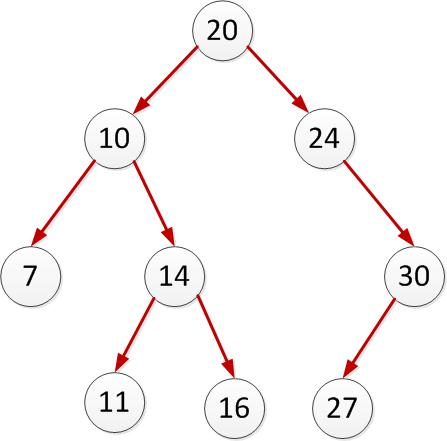
\includegraphics[width=3in, height=3in]{Figures/Figure14}}
  \end{center}
  \centering
	\parbox{3in}{\caption{A binary tree.} \label{fig14}} 
\end{figure}

\section{AVL Tree}

The Line Sweep Algorithm uses an AVL tree instead of a binary tree. The AVL tree is named after its two Soviet inventors, G. M. Adelson-Velskii and E. M. Landis, who published it in their 1962 paper ``An algorithm for the organization of information". \cite{AVL} An AVL tree is pretty much similar to a binary search tree except for the fact that it is a self-balancing binary search tree. The AVL tree is named after its two inventors, G.M. Adelson-Velskii and E.M. Landis. In an AVL tree the heights of two child subtrees of any node differ by at most one. The insertion or deletion operations on an AVL tree may require the tree to be rebalanced by one or more tree rotations.

The balance factor of each node is the height of its left subtree minus the right subtree. Sometimes this can be opposite but in our implementation it is the height of the left subtree minus the right subtree. This height is stored in each node and kept updated at any particular instance of time. A node with a balance factor of 1, 0 or -1 is considered as balanced. In other words we perform rotation operations whenever the balance factor of any node becomes either 2 or -2. In these situations we perform the rotation operations in order to balance the AVL tree.

\section{Special Algorithm Requirement}

In our implementation, according to the text book \cite{TEXTBOOK1} we store some special data in each internal node. Each internal node stores the right-most child in its left subtree. Theoretically each internal node should store some data that guides the path to the destination node where the actual data is stored. So instead of storing the segments in internal nodes we store the right most segment in its left subtree. While finding a particular segment we test if the segment lies to the left or right of the segment stored in the internal node and descend accordingly based on the outcome. Eventually we would reach the leaf node. Each Update and Delete operation takes {\it O}(log n) time.

\section{Tree Rotations}

Tree rotations are done mainly in order to balance the tree. There are primarily two kinds of tree rotations namely left rotation and right rotation. These rotations are pictorially represented in the Figure.~\ref{fig15}.
\begin{figure}[ht]
  \begin{center}
   	\fbox{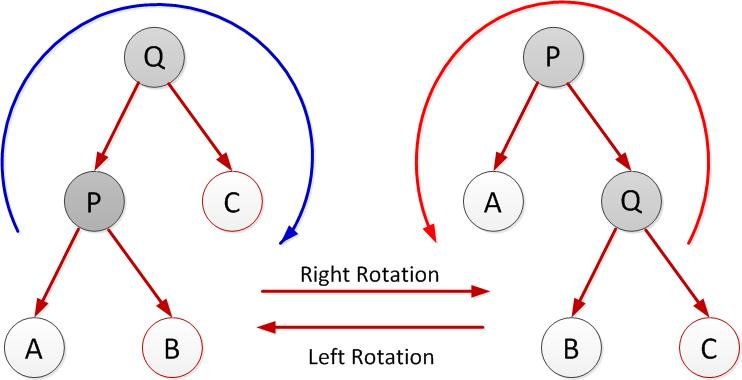
\includegraphics[width=5in, height=2.5in]{Figures/Figure15}}
  \end{center}
  \centering
	\parbox{5in}{\caption{Left and right rotations of a tree.} \label{fig15}} 
\end{figure}

The right rotation operation is performed in Figure ~\ref{fig15} with Q as the root. This operation results in a tree structure as shown on the right side by performing rotation in clockwise direction of the tree shown on the left side. Similarly the left rotation is performed in the inverse direction rooted at node P. This results in a tree structure as shown in the left side by performing rotation on anticlockwise direction of the tree shown on right side. There are a few rules that must be followed while performing rotations. These rules are -
\begin{enumerate}
	\item The order of the leaves prior to rotation and post rotation must remain the same. In other words the order of the leaves in the depth first search should remain the same before and after the rotation.
	\item For any particular node the right child must always be greater than or equal to the parent node and the left child must be less than the parent node. This is the basic property of a binary search tree which needs to be followed by tree rotations.
\end{enumerate}

It thus implies that the leaf nodes can change the parent nodes after rotation but they still follow the two rules stated above. Both the left and right rotations should preserve the integrity of the tree which balancing the tree.

\section{Importance of balacing a tree}

If we do not balance the tree then either the left or right subtree will continue to increase at an exponential rate than the other corresponding subtree. This can significantly affect the performance for lookup and would become linear in the worst case scenario. If only the left or right subtree continue to grow then the data structure would no longer be a tree but would be a linked list.

\section{Tree rotations in order to balance a tree}

As we stated before a tree rotation is performed as soon as the balance factor of any node becomes either 2 or -2. If we interpret the meaning of the balance factor of 2 or -2 then it can be easily understood that either the left or the right subtree is 2 nodes greater in height than the other corresponding subtree. If this were not the case then the balance factor would never be 2 or -2. When a subtree is rotated, the subtree side upon which it is rotated decreases its height by one while the other subtree increases its height by one. This makes tree rotations as a useful tool in rebalancing the tree. There are four conditions that can cause the rotation of tree to be triggered.  In some scenarios only a single rotation will not rebalance the tree. Consider the left right and the right left case as given in Figure.~\ref{fig16} \cite{TREEROTWIKI}. In the case of the left right case initially a left rotation is performed on the right child of the left child of node whose balance factor triggered the rotation so that the tree structure becomes like a left left case. Then again a right rotation is performed on the node that triggered the rotation. Similarly corresponding opposite steps is performed for a right left case. Note that these extra steps are taken so that the rotations follow the two rules stated previously in this chapter in order to maintain the integrity of the tree. The steps can be summarized by a small table, given by Table \ref{tab1}.
\begin{figure}[ht]
  \begin{center}
   	\fbox{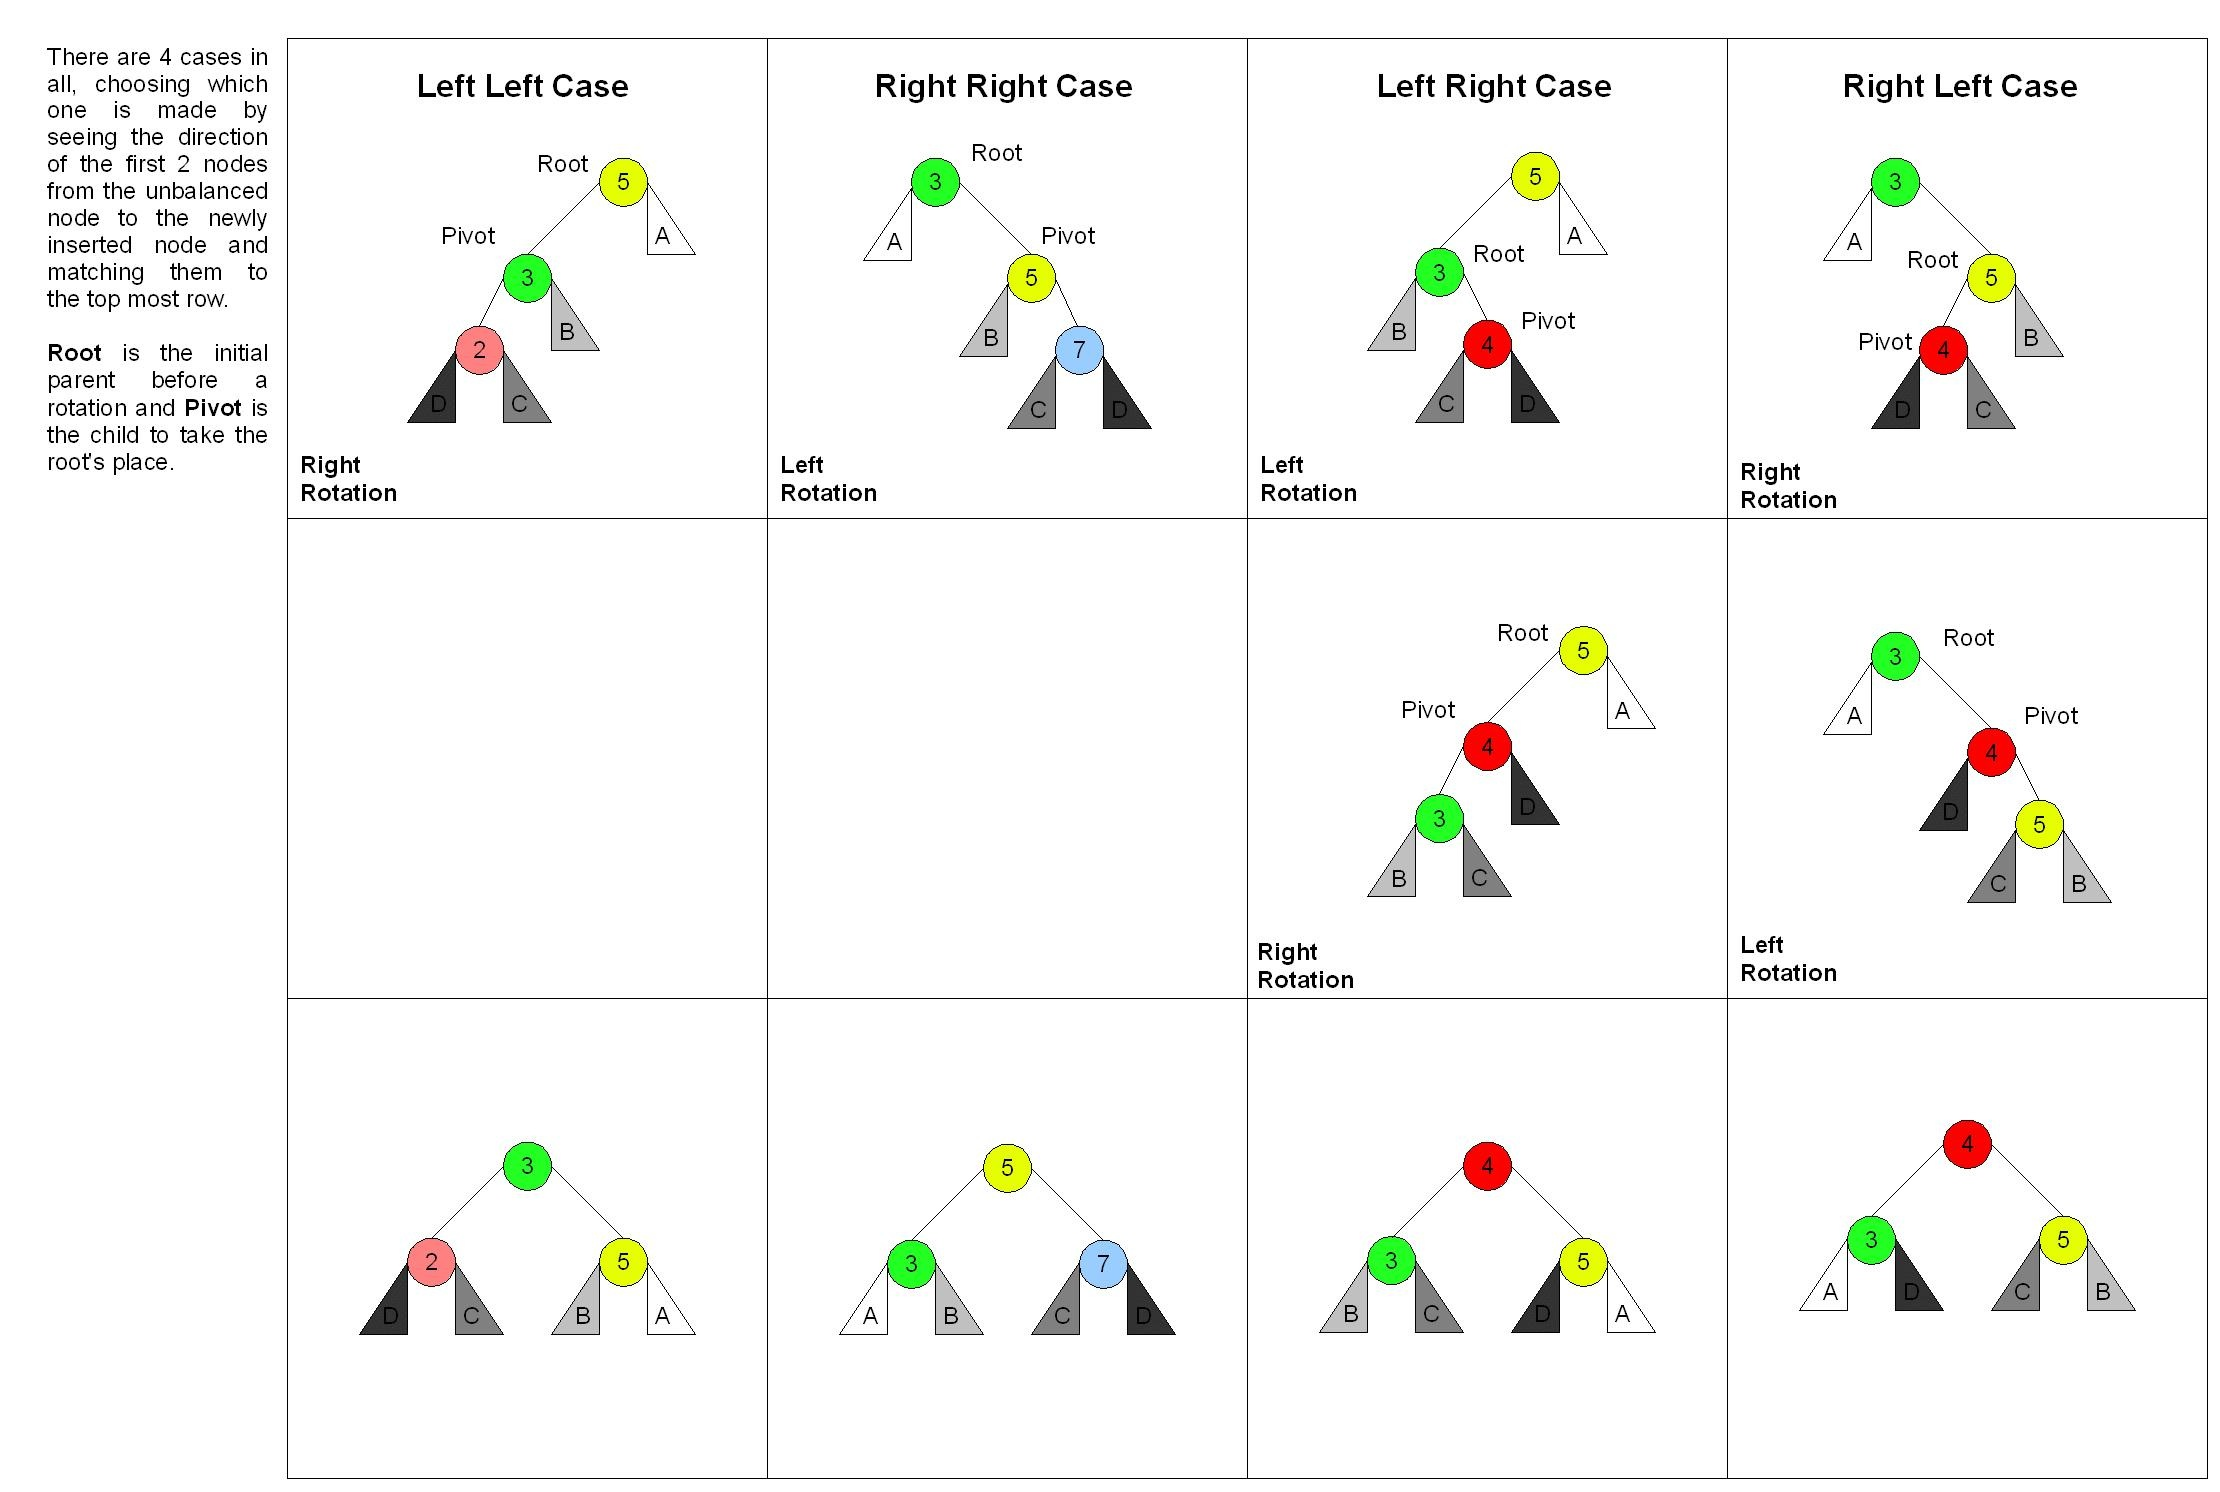
\includegraphics[width=6.5in, height=7in]{Figures/Figure16}}
  \end{center}
  \centering
	\parbox{6.5in}{\caption{Pictorial representation of rotations causing rebalancing in an AVL tree. Source: WIKIPEDIA, \textbf{\textit{Tree balancing - Wikipedia, the free encyclopedia}}. Tree Rebalancing, http://en.wikipedia.org/wiki/File:Tree Rebalancing.gif, accessed Aug. 2012, n.d.} \label{fig16}} 
\end{figure}

\clearpage
\begin{table}[hbt]
\centering
  \begin{minipage}{5in}
    \caption{Steps Required to Balance Tree After Node Insertion\label{tab1}}
    \begin{tabular}{||p{2.5cm}|p{2.5cm}|p{2.5cm}|p{4.5cm}||}    \hline
      Node Balance Factor &	Left Subtree Balance Factor  &  Right Subtree Balance Factor & Steps \\ \hline \hline
      -2 & - & -1  & Perform Left Rotation \\ \hline
	  -2 & - & 1  & Perform Right Rotation and Perform Left Rotation \\ \hline
	   2 & 1 & -  & Perform Right Rotation \\ \hline
       2 & -1 & -  & Perform Left Rotation and Perform Right Rotation \\ \hline
    \end{tabular}
  \end{minipage}
\end{table}

The rotation operations, given in Table \ref{tab1} are triggered whenever a particular node is deleted. Besides these operations there is one more additional step that needs to be performed which is specific only when a node is deleted from a tree, given by Table \ref{tab2}. These operations are specifically executed whenever a particular node is deleted from an AVL tree. (Note that these are the additional operations, which needs to be performed along with the operations given in Table \ref{tab1}).
\begin{table}[hbt]
\centering
  \begin{minipage}{5in}
    \caption{Extra Steps Required to Balance Tree After Node Deletion\label{tab2}}
    \begin{tabular}{||p{2.5cm}|p{2.5cm}|p{2.5cm}|p{4.5cm}||}    \hline
      Node Balance Factor &	Left Subtree Balance Factor  &  Right Subtree Balance Factor & Steps \\ \hline \hline
      -2 & 0 & -  & Perform Right Rotation \\ \hline
	   2 & - & 0  & Perform Left Rotation and Perform Left Rotation \\ \hline
	\end{tabular}
  \end{minipage}
\end{table}

The concepts, rules and operations mentioned until now are the general AVL tree rule�s that needs to be followed by any implementation of an AVL tree. The advanced line sweep algorithm also has one more additional rule that needs to be followed. Each internal node needs to store the right most child node in the left subtree. This rule is extremely challenging to be followed because this is the only thing that is mentioned about the rule in the text book [1]. There is no implementation details stated as to how this rule should be followed. This is also challenging because the internal nodes also needs to be adjusted whenever a particular node is inserted or deleted from the AVL tree. The implementation needs to make sure that the tree rotation does not violate this rule. Thus one more rule has been added besides the two previous rules for tree rotation. We manage to maintain the integrity of the whole tree along with the internal node rules. This is not a trivial task and it took me almost a month to come up with the solution. I have narrowed down the task by breaking it into finite number of steps so that it can be easy to program.

\section{Tree Node Insertion}
\begin{enumerate}
	\item No special thing as such needs to be done when inserting the root node.
	\item If the new node is being inserted as the left node of an already existing node (parent node) and there is no right child for the parent node (Figure.~\ref{fig17}) then insert a new node as the parents right child with the data same as the parent node and copy the data of the left child to the parent node. For instance in Figure ~\ref{fig17}, a new node 2 was inserted to the left of node 4 since 2 is less than 4. Then we created a new node with the same data as the root node as inserted it to the right of the parent node. Also we changed the data of the root node to be the same as the left node�s data.
	\item There would never be a situation where the new node is being inserted as the left node of an already existing node (parent node) and there is an existing right child of the parent node.
	\item Similarly there would never be a situation where the new node is being inserted as the right node of an already existing node (parent node) and there is an existing left child of the parent node.
	\item Rules 3 and 4 hold true because we will always insert/ delete a leaf node and adjust the other corresponding node during insertion/ deletion.
	\item If the new node is being inserted as the right node of an already existing node (parent node) and there is no left child of the parent node (Figure.~\ref{fig18}) then simply insert the new node as the right child of the parent node and insert a new left child of the parent node having the same data as the parent node. Also we need to copy the data of the right child of the parent to the parent of its left most parent. This step will make sure that the internal node is also adjusted properly.
\end{enumerate}
\begin{figure}[ht]
  \begin{center}
   	\fbox{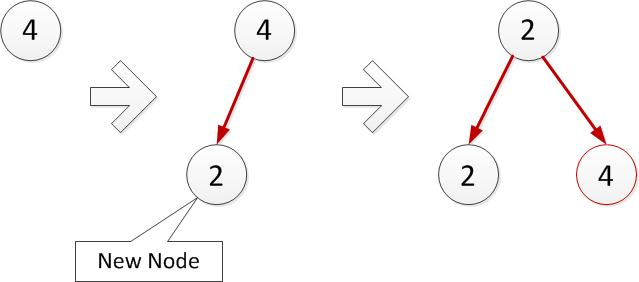
\includegraphics[width=5in, height=2in]{Figures/Figure17}}
  \end{center}
  \centering
	\parbox{5in}{\caption{Inserting a new left leaf node.} \label{fig17}} 
\end{figure}
\begin{figure}[ht]
  \begin{center}
   	\fbox{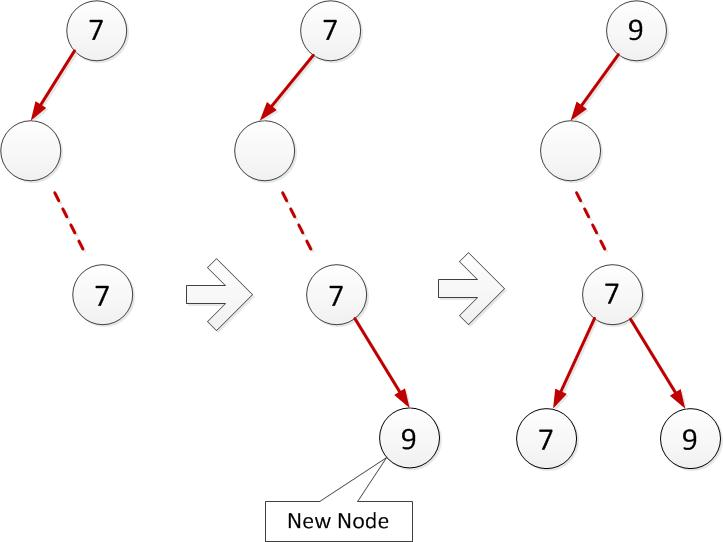
\includegraphics[width=5in, height=3in]{Figures/Figure18}}
  \end{center}
  \centering
	\parbox{5in}{\caption{Inserting a new right leaf node.} \label{fig18}} 
\end{figure} 
\section{Tree Node Deletion}
\begin{enumerate}
	\item If we are deleting the root node explicitly (not in order to maintain the internal nodes) then it should be the only node in the tree. In other words when we are deleting the root node explicitly then it should not have any children.
	\item If the node that we are deleting is a left child and its parent is a root node (Figure.~\ref{fig19}) then it implies that the root node�s data and its left child (the node to be deleted) are the same. Hence we delete both the root node and its left child and make the root node�s right child as the new root node.
	\item If the node that we are deleting is a left child of some parent node (Figure.~\ref{fig20}) and that parent node is not a root node then we delete both the parent node and its left child (the node that we wanted to delete originally) and set the parent�s right child as the child of the parents parent node. This right child would be a right child if the parent node was also a right child of its parent otherwise it would be a left child.
	\item If the node that we are deleting is a right child of some parent (Figure.~\ref{fig21}), then we get its left most parent node. The parent node of its left most parent node must be equal to the node that we want to delete. Hence we delete the parent of the left most parent node and the node that we want to delete and adjust pointers accordingly.
	\item Each time we make adjustment, we need to make sure that the root node is updated correctly if needed and that the AVL tree follows the basic 3 rules stated earlier in this chapter.
\begin{figure}[ht]
  \begin{center}
   	\fbox{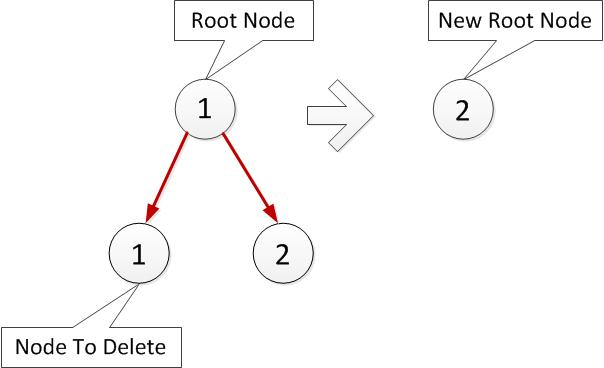
\includegraphics[width=4.5in, height=2.5in]{Figures/Figure19}}
  \end{center}
  \centering
	\parbox{4.5in}{\caption{Deleting left child of root node of height one.} \label{fig19}} 
\end{figure}
\begin{figure}[ht]
  \begin{center}
   	\fbox{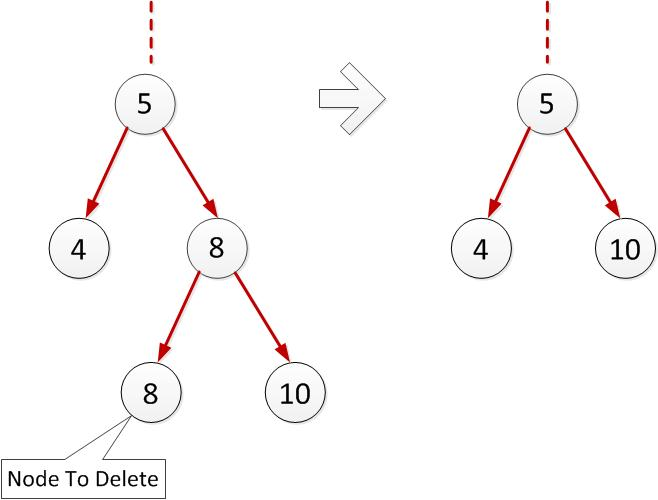
\includegraphics[width=4in, height=2.30in]{Figures/Figure20}}
  \end{center}
  \centering
	\parbox{4in}{\caption{Deleting a left leaf.} \label{fig20}} 
\end{figure}
\end{enumerate}
\begin{figure}[ht]
  \begin{center}
   	\fbox{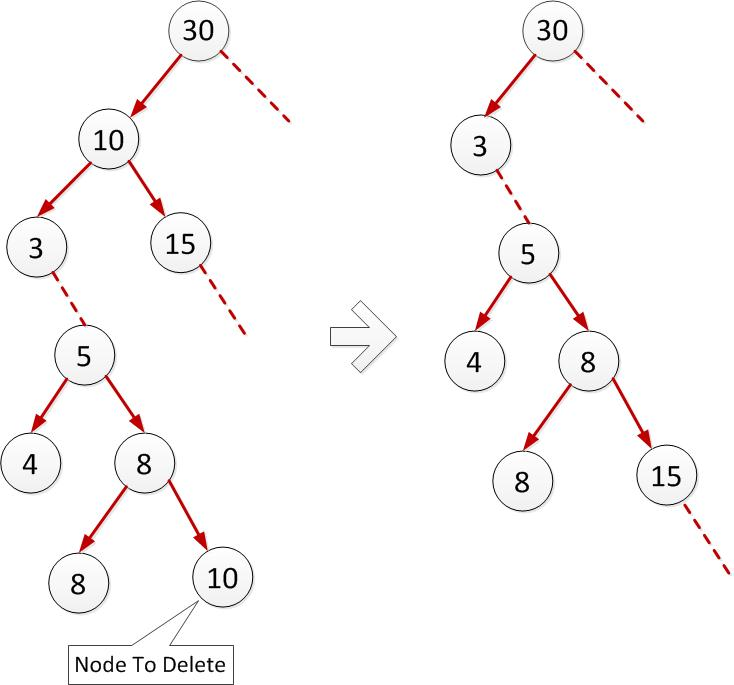
\includegraphics[width=4in, height=4.5in]{Figures/Figure21}}
  \end{center}
  \centering
	\parbox{4in}{\caption{Deleting a right leaf.} \label{fig21}} 
\end{figure}

It is a very important point to be worth noted that each time a node is inserted or deleted then the balance factor must be calculated for all the nodes starting from the inserted node or the parent of the deleted node up to the root node and rotations be performed if needed in order to balance the tree.
% Note that if you want something in single space you can go back and
% forth between single space and normal space by the use of \ssp and
% \nsp.  If you want doublespacing you can use \dsp.  \nsp is normally
% 1.5 spacing unless you use the doublespace option (or savepaper
% option)
%
%(FORMAT) Usually you *don't* want to mess with the spacing for your
%(FORMAT) final version.  If you think/know that the thesis template
%(FORMAT) and/or thesis style file is incorrect/incomplete, PLEASE
%(FORMAT) contact the maintainer.  THANK YOU!!!

\chapter{ESSENTIAL CONTRIBUTIONS OF THIS THESIS}
\label{chap:binarysearchtree}
% By labeling the chapter, I can refer to it later using the
% label. (\ref{chap:binarysearchtree}, \pageref{chap:binarysearchtree}) Latex will take care
% of the numbering.

\section{Crux of the thesis} 

The main research topic of this thesis is to optimize the time required to compute the neighnor in an AVL tree. We have studied uptil now the original algorithm as given in the text book \cite{TEXTBOOK1}. One of the goals of this thesis research is to present a traditional working algorithm for academic purpose. Also besides implementing the original algorithm, the main contribution of this thesis research is to modify one of the data structure used in to original algorithm with an intention to optimize it. By doing so we will present an optimized version of the algorithm.

As we have already seen till now we are using an AVL tree to maintain the status structure and event queue. One of the most frequently required operations for these data structures is to compute the adjacent left and right neighbor�s. With the traditional implementation of an AVL tree suppose we search in the tree for the segment immediately to the left of some segment �L1� that lies on the sweep line. At each internal node �V� starting from root node we first need to find the leaf node �L1�. Thus at each internal node �V� we test whether �L1� lies to the left or right of the segment stored at the internal node. Depending on the outcome we descend to the left or right of the segment stored at �V� eventually ending up in the leaf node �L1�. Now since we need to find the left neighbor of �L1� we first need to traverse to the common parent between �L1� and its left neighbor. After that we need to descend downwards to get the left neighbor of �L1�. Similar strategy is to be followed but exactly in the opposite direction for finding the next right neighbor. This would take{\it O}(log n) time and is a very costly operation. This would be worst if the neighbor lies in an entirely different subtree and would require us to traverse back to the root and then descend again downwards in the direction of the neighbor.
\begin{figure}[ht]
  \begin{center}
   	\fbox{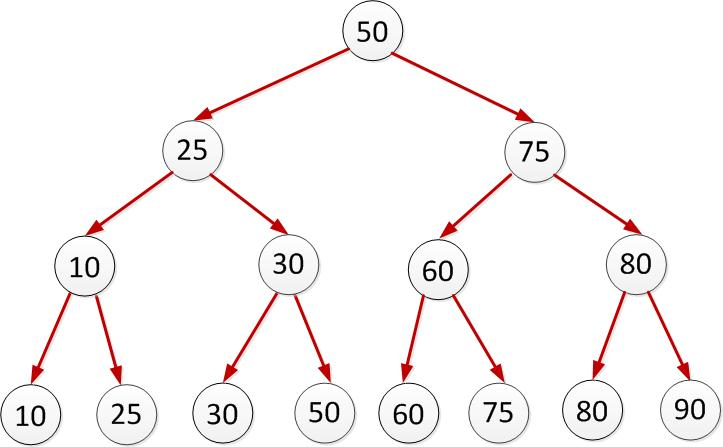
\includegraphics[width=6in, height=2.75in]{Figures/Figure22}}
  \end{center}
  \centering
	\parbox{6in}{\caption{A typical balanced AVL tree.} \label{fig22}} 
\end{figure}

For instance consider Figure.~\ref{fig22}. Suppose we need to find the left neighbor of 50. We would start with the root node 50 and descend towards left as search node �50� is equal to the root node 50. Then we would come at node 25. After which we would move right downward as 50 is greater than 25. Thus we would reach node 30 and finally at 50 which is the leaf node. But we wanted to get the left neighbor of 50, so we would again move upward to 30 which happen to be the common parents between leaf node 50 and its left neighbor. Then we would move down left to get 30, which is the left neighbor, which is the actual node that we were searching. Now suppose we wanted to find the right neighbor of 50 then we would start at root node and traverse 50-25-30-50 as before. But since we wanted the right neighbor, we would have to first traverse to the common parent between leaf node 50 and its right neighbor.  Thus we would again traverse all the way upwards starting at leaf node 50 with the path 50-30-25-50 and then move right to follow the path 75-60-60 to finally get the right neighbor of 50. This would be a very costly operation if the depth of the tree is huge.

It would certainly be better if we could optimize this time as this is the most frequently used operation in the algorithm. This thesis is proposing an elegant solution where this searching can be optimized. As the tree is built this thesis proposes to store the left and right pointers only in the leaf nodes. These pointers would be continuously updated whenever a new node is inserted or deleted in the tree (Figure.~\ref{fig23}).  
\begin{figure}[ht]
  \begin{center}
   	\fbox{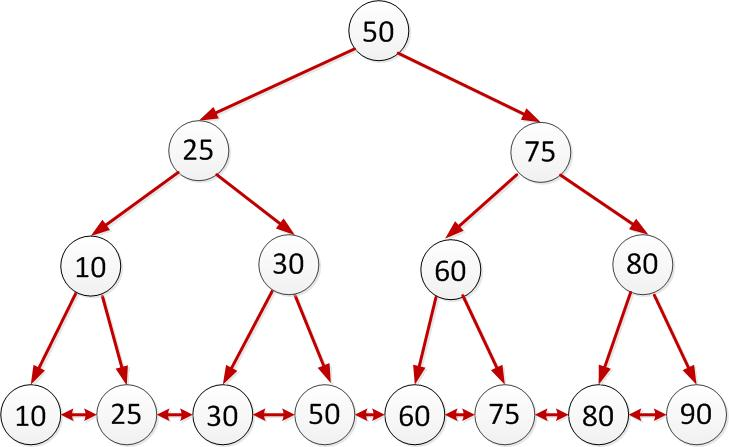
\includegraphics[width=6in, height=2.75in]{Figures/Figure23}}
  \end{center}
  \centering
	\parbox{6in}{\caption{Optimized balanced AVL tree.} \label{fig23}}
\end{figure}

These pointers would be gradually built as the tree grows and there is no separate routine which will update these pointers. These pointers building/ maintaining operation would be built in the tree formation itself. The only thing we should be careful is to update these pointer whenever a node is inserted into or deleted from the tree. Suppose we inserted a new node 55 in between 50 and 60 then the right pointer of 50 and left pointer of 60 should point to 55. At the same time the left pointer of 55 should point to 50 and the right pointer of 55 should point to 60 (Figure.~\ref{fig24}). Similarly while deleting node 55 which was inserted in previous step we need to make sure that right pointer of node 50 points to 60 and the left node of point 60 points to 50.
\begin{figure}[ht]
  \begin{center}
   	\fbox{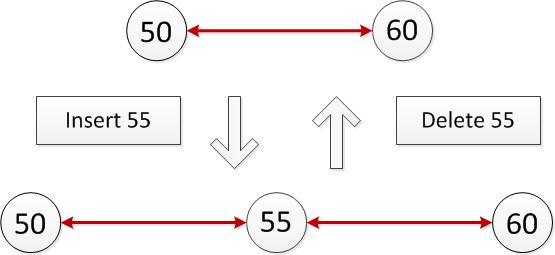
\includegraphics[width=6in, height=1.75in]{Figures/Figure24}}
  \end{center}
  \centering
	\parbox{5in}{\caption{Inserting a leaf in-between two leaves in an optimized AVL tree.} \label{fig24}} 
\end{figure}

\section{Tree rotations}
Remember, we need to perform tree rotations when the tree is not balanced in order to balance it. We perform left or right rotation or a combination of both in a certain order in order to balance the tree. Initially it may seem that maintaining these proposed tree pointers would be a night mare when the tree rotation(s) is performed. All the left and right pointers would seem to be messed when the tree is rotated. Surprisingly, as a matter of fact we do not need to do any special operation when the tree is rotated. If we recall the rules stated for performing tree rotations as given below.
\begin{enumerate}
	\item The order of the leaves prior to rotation and post rotation must remain the same. In other words the order of the leaves in the depth first search should remain the same before and after the rotation.
	\item For any particular node the right child must always be greater than or equal to the parent node and the left child must be less than the parent node. This is the basic property of a binary search tree that needs to be followed by tree rotations.
\end{enumerate}

The first rule is the answer to the question that we just presented. The tree rotation follows the order of the leaves of the tree from left to right or vice-versa. Thus the tree rotation should just work as is without modifying it. If the leaves of the tree maintain the order pre and post rotation then there is no need to update the left and right pointers maintained in the leaves of the tree.

\section{Good Geometric Algorithm}

What makes a geometry algorithm good?  One factor is that it correctly solves a significant problem.  If an algorithm is the very first one or the only one to solve a certain problem, then that alone would make it significant.  Otherwise, something else has to distinguish it.  The primary theoretical  criterion used to compare algorithms is their efficiency, especially their asymptotic efficiency (aka ``computational complexity") as the size n of the problem involved becomes increasingly large,  given by Table \ref{tab3} \cite{SOFTSURFER}.  That is, the algorithm has to be ultimately faster than the competition.  Beyond speed, additional secondary criteria for good algorithms include: the amount of storage space they use, their runtime efficiency for low values of n, their ease of implementation, and also the sheer elegance of the algorithm's solution.  In some cases, the secondary criteria can outweigh the primary one.  For example, in a 1990 tour-de-force, Chazelle described a linear time {\it O}(n) algorithm for triangulating a simple polygon in the plane \cite{Chazelle}.
\begin{table}[hbt]
  \begin{minipage}{6in}
    \caption{Time Complexity of An Algorithm For Input `n'\label{tab3}}
    \begin{tabular}{||p{1.5cm}|p{2cm}|p{2cm}|p{2cm}|p{2cm}|p{2cm}|p{2cm}||}    \hline
      logn & n & nlog n & $n^{2}$ & $n^{3}$ & $n^{4}$ & $2^{n}$ \\ \hline \hline
      0 & 1 & 0 & 1 & 1 & 1 & 2 \\ \hline
	  1 & 2 & 2 & 4 & 8 & 16 & 4 \\ \hline
	  2 & 4 & 8 & 16 & 64 & 256 & 16 \\ \hline
	  3 & 8 & 24 & 64 & 512 & 4096 & 256 \\ \hline
	  4 & 16 & 64 & 256 & 4096 & 65536 & 65536 \\ \hline
	  5 & 32 & 160 & 1024 & 32768 & 1048576 & 4294967296 \\ \hline
	  6 & 64 & 384 & 4096 & 262144 & 16777216 & xxxxxxxxxx \\ \hline
	  7 & 128 & 896 & 16384 & 2097152 & 268435456 &  \\ \hline
	  8 & 256 & 2048 & 65536 & 16777216 & 4294967296 &  \\ \hline
	  9 & 512 & 4608 & 262144 & 134217728 & xxxxxxxxxx &  \\ \hline
	  10 & 1024 & 10240 & 1048576 & 1073741824 &  &  \\ \hline
	  15 & 32768 & 491520 & 1073741824 & xxxxxxxxxx &  &  \\ \hline
	  20 & 1048576 & 20971520 & xxxxxxxxxx &  &  &  \\ \hline
	  25 & 33554432 & 838860800 &  &  &  &  \\ \hline
	\end{tabular}
	\begin{minipage}{1.09\linewidth}
  \begin{tablenotes}[para, flushleft] Source: SOFTSURFER, \textit{Softsurfer}. Geometry Algorithms, \newline http://www.softsurfer.com/overview.htm, accessed Aug. 2012, n.d.
  \end{tablenotes}
  \end{minipage}
  \end{minipage}
\end{table}
However, to this day that algorithm has never been implemented because it is too complicated!  So, other triangulation algorithms that are both reasonably fast and easy to implement become significant.  On the other hand, finding a way to simplify Chazelle's algorithm and actually programming it would be of great significance \cite{SOFTSURFER}.

\section{Space Complexity}

We would need to have extra space of two double words (DWORD), In other words we would need to have 8 bytes $=$ 64 bits for each leaf node in order to save the left and right pointers. Thus in total we would need 64 $*$ n bits more or 8 $*$ n bytes than the original implementation. The important point is that we only store the left and right pointers in the leaf nodes and hence we don`t need the extra space for the internal nodes. Also conceptually the internal nodes should only store the information required to guide the search. The time that we save by following this approach certainly accounts for the extra space.

\section{Time Complexity}

This new approach to save the extra left and right pointers would take constant time to be maintained as they are gradually built as the tree grows. There is no separate dedicated method or loops which will maintain these pointers. They are built into the algorithm and hence would be constant which we can ignore. 
The neighbor search operation for a typical AVL tree takes {\it O}(log n) time \cite{BST}. The neighbor search operation in the optimized mode of the algorithm requires to access the value stored in the left and right pointers only. Thus these are primitive operation and does not include any kind of loops or accessing complex data structures. Hence the neighbor search operation in the optimized mode of the algorithm would require constant time {\it O}(1) time. Thus it is clearly a huge improvement especially for large trees. This would save tremendous amount of time in finding the neighbor when this algorithm is used in some real world application, where the number of input lines are huge.

% Note that if you want something in single space you can go back and
% forth between single space and normal space by the use of \ssp and
% \nsp.  If you want doublespacing you can use \dsp.  \nsp is normally
% 1.5 spacing unless you use the doublespace option (or savepaper
% option)
%
%(FORMAT) usually you *don't* want to mess with the spacing for your
%(FORMAT) final version.  If you think/know that the thesis template
%(FORMAT) and/or thesis style file is incorrect/incomplete, PLEASE
%(FORMAT) contact the maintainer.  THANK YOU!!!

\chapter{IMPLEMENTATION}
\label{chap:chapter5}
% by labeling the chapter, I can refer to it later using the
% label. (\ref{chap:chapter5}, \pageref{chap:chapter5}) Latex will take care
% of the numbering.

\section{Technology Used}

The line sweep algorithm has been developed purely in C++ language without any dependency on any third party library. Although this algorithm could have been implemented in any language or platform of choice, C++ was selected because of its high performance and easy pointer manipulation. The program was tested successfully on Windows platform. The development was initially started using Visual Studio 2008 but later upgraded to Visual Studio 2010 and finally to Visual Studio 2012 RC. The visual studio solution for this program has already been statically linked with Microsoft Foundation Library (MFC) and Active Template Library (ATL) Component Object Model (COM).

\section{Implementation Details}

I have tried to follow the best coding practices while implementing the algorithm and have made heavy use of C++ templates while coding the algorithm. Even though the status structure and event queue are two different data structures used for entirely different purpose, the C++ class for them is just one and has only one implementation. This C++ class for AVL tree has been written as a template based class. Event Queue and Status Structure are actually different C++ structures which are provided as template parameters to the AVL tree class. This is the first time I have made use of C++ template on such a large scale and understood the true power of it. Without C++ templates the code for this algorithm would have been unnecessarily bloated and would have been hard to develop and maintain. Below is the sample snippet of the actual header definition of the AVL tree class.

\noindent
template $<$typename TREETYPE$>$ \newline
class CAVLTree \newline
\{ \newline
\hspace*{2em} private: \newline
    		\hspace*{4em} $CAVLTreeNode<TREETYPE>* m\_pRoot;$ \newline
\hspace*{2em} public: \newline
    		\hspace*{4em} // Constructor \newline
		     \hspace*{4em} CAVLTree(void); \newline
    		\hspace*{4em} // Destructor \newline
    		\hspace*{4em} virtual ~CAVLTree(void); \newline
\hspace*{2em} . \newline
\hspace*{2em} . \newline
\hspace*{2em} . \newline
\}

The above code snippet should give a little bit idea of the implementation details. It can be seen from the code that it follows Hungarian naming convention \cite{HUNGARIAN} which makes the program more readable. One more contributing factor to the code being more readable and easy to interpret is the considerable usage of operator overloading. Operator overloading is a powerful feature of C++ by which we can redefine what operators do and how they behave under certain circumstances. For instance, consider the CAVLTreeNode class, which represents a node in an AVL Tree and suppose that it had a public method as given below -
 
\noindent
Class CAVLTreeNode \newline
\{ \newline
\hspace*{2em} public: \newline
	\hspace*{4em} bool IsLessThan(CAVLTreeNode objNodeToCompareWith); \newline
\}

The above method ``IsLessThan" determines if a node object is less than the other node object that is passed as a parameter. Instead of the above way of coding, this thesis project makes use of operator overloading in the below manner.

\noindent
Class CAVLTreeNode \newline
\{ \newline
\hspace*{2em} public: \newline
	\hspace*{4em}  bool operator $<$ (CAVLTreeNode objNodeToCompareWith); \newline
\}

This way it more easy to understand the calling code since it would call, just as we would imagine the normal way of writing obj1 $<$ obj2 rather than obj1.IsLessThan(obj2). The code has also been tested so that it works on Multi-Byte Character set as well as Unicode Character set. All the strings have been stored in resource file so that it should be easy to run the program in a different locale if proper translations are available for the string in a different �Resource only� DLL.

The project has been programmed to generate the lines using random number generator. User would just need to input the total number of lines he/ she wants to run the program with and the program would automatically generate those numbers of lines and perform line sweep algorithm on it. This feature would be very useful if the user wants to see the demonstration of the working of the program on a huge number of lines like 100 or even 1000. That way the user won�t have to manually input the co-ordinate points of those lines. If the user would have to do it manually then it would be imperative to input two set of points for each line, namely the upper point and the lower point. Likewise for 100 and 1000 lines the user would have to input 200 and 2000 points respectively which sounds quite laborious and thus prone to errors. When the GUI for this algorithm is done then it might be a good idea to let the user draw lines using mouse so that the user can give whatever input he/ she wishes.

The algorithm works in two modes. One is the classic algorithm mode as given in the text [1] and the other mode is known as the optimized mode. In optimized mode the algorithm would run with the optimization as stated in the previous chapter where all the leaf node�s would contain the pointers to their left and right neighbors so that the neighbor search operation could be done in constant time instead of {\it O}(log n) time. The two modes of the algorithm can be toggled with the help of a single globally scoped Boolean variable named g\_bOptimizedMode which is defined in ``Globals.cpp" file. To enable the optimized mode we would have to just set the Boolean value to true (g\_bOptimizedMode = true). That would enable the optimized mode and setting the variable to false would disable the optimized mode (g\_bOptimizedMode = false). This behavior can be easily wrapped up in a function so that an intuitive button can be provided to toggle between the two modes of the program. The program can be run in either mode without recompiling. The thesis project has been architected and designed in such a way that giving a GUI to the program should be very easy with least modifications as possible.

\section{Lessons Learnt}

The source code for this thesis project as well the documentation is version controlled using SVN version control software which is freely available as open source software. Proper versioning helps to make sure that the source is properly backed up at one place and also the actual difference can be seen in the source code for different versions. It is very easy and convenient to pull a back copy of a certain file. Version controlling will also make it easy to distribute the code with other users if needed in future. At the very beginning the thesis project was not using any version control software and later it became very hard to manage the code and take backup as the code started increasing which eventually made it imperative to use SVN. SVN was the choice made as it is freely available, open source, popular and in-fact used by many open source software projects, currently being worked upon by hundreds and thousands of developers worldwide.

The most important lesson learnt while developing the thesis project was to not underestimate the importance of memory management. The first working model of the project was working perfectly fine and was returning proper output until when I used CRT runtime library to find out if my program was having any memory leaks. I anticipated that the program would not have any leaks since I was releasing any explicitly allocated memory at proper places and in destructors. To my surprise when I debugged, I found out that the program was leaking 143 kb of memory which was a very small leak. I had the option to leave the program as it is since it was running perfectly fine but somehow it did not appeal me since I knew that there was problem somewhere in the program and it was my duty to fix it even though it might not be profiting me right away. I spend around 2 weeks debugging and trying to fix the memory leaks just so that I would be happy with myself of having fixed the problem. The process of finding the leaks was not so easy. I had to scan and understand the dump statistics of the leaked memory returned by CRT runtime. The more interesting part was that the leaks started increasing as I was trying to solve it. It increased from 143 kb to 180 kb, 350 kb and the highest it went was up to 810 kb. It wasn�t clear if the decision to fix the memory leak was right. I eventually ended up rewriting 60\% of the code. I literally rewrote the module that performs tree rotation, insertion and deletion which was the core code of the research project. I found out that there were some serious bugs in the program even though it was giving out the right output. Surprisingly the tree rotation code was performing the rotation but was incorrectly handling pointer manipulation, as a result of which some nodes were left hanging out orphaned which was causing the memory leak. Even though the output was correct the internal data structure of Event Queue and Status Structure was incorrect. The program generating correct output was a matter was luck and might have failed with some other input. Hence the decision to fix memory leaks was certainly fruitful even though the result was not evident upfront when I took the decision to fix it. Thus the biggest lesson learnt was to never underestimate the memory leaks in the program no matter even if it a small one. There are several good articles and videos out on MSDN which could be useful in understanding the techniques and API�s required in order to find memory leaks. Read MSDN memory leak topic on http://msdn.microsoft.com/en-us/library/x98tx3cf(v=vs.71).aspx.

\section{Architecture}

The code for the thesis project has been architected using the concepts learnt in software architecture class so that the code is easy to develop and maintain further with least modifications as possible. There are basically 6 classes as stated below with a short description of them.
\begin{enumerate}
\item CAlgorithm: This class represents the algorithm as the name rightly suggests. This class contains the core logic of the algorithm. The main function which starts the program, interacts with this class. 
\item CAVLTree: This class represents the tree and contains the code to handle all the tree related operations such as insertion, deletion, left rotation, right rotation etc.
\item CAVLTreeIterator: This is the iterator class, which provides helper functions to iterate through the tree.
\item CAVLTreeNode: This is the class, which represents each node of an AVL tree and provides function specific to each node.
\item CEventQueueData: This class represents the Event Queue and has methods specific to the Event Queue.
\item Cline: This class represents a line in a Euclidian Space.
\end{enumerate}

In general the main function interacts with the �CAlgorithm� class. It creates an object of �CAlgorithm� class, which represents an instance of the algorithm. The algorithm then creates two objects of CAVLTree class. One of them represents the Event Queue and the other represents the Status Structure. An object of �CAVLTreeNode� class represents each node of the tree. The algorithm uses �CAVLTreeIterator� whenever it wants to iterate through the tree. Also an object of the �Cline� class would represent each line used thought the algorithm.

The program makes user of the iterator design pattern and hence it has a CAVLTreeIterator class which provides helper methods in iterating through the AVL tree. The classes are loosely coupled with each other so that modification of one class does not affect the other. Also the program makes use of the a global macro defined again in the precompiled header file �stdafx.h� namely SAFEDLETE and SAFEDELETEARRAY which are used throughout the program to delete memory explicitly assigned on the heap.

% Note that if you want something in single space you can go back and
% forth between single space and normal space by the use of \ssp and
% \nsp.  If you want doublespacing you can use \dsp.  \nsp is normally
% 1.5 spacing unless you use the doublespace option (or savepaper
% option)
%
%(FORMAT) usually you *don't* want to mess with the spacing for your
%(FORMAT) final version.  If you think/know that the thesis template
%(FORMAT) and/or thesis style file is incorrect/incomplete, PLEASE
%(FORMAT) contact the maintainer.  THANK YOU!!!

\chapter{RESULTS AND DISCUSSION}
\label{chap:resultsdiscussion}
% by labeling the chapter, I can refer to it later using the
% label. (\ref{chap:resultsdiscussion}, \pageref{chap:resultsdiscussion}) Latex will take care
% of the numbering.

\section{Sample Output}
This section presents a sample output run of the program for input as given in Figure.~\ref{fig25}. This input has been specifically choosen since it contains odd cases like vertical lines, horizontal lines, lines having intersection points as the starting point of other line, a single line which intersects 2 or more lines.
\begin{figure}[ht]
  \begin{center}
   	\fbox{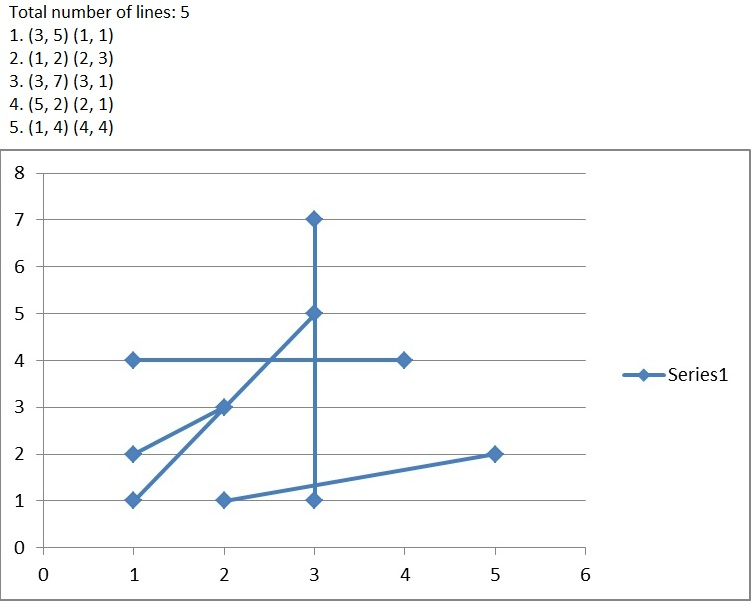
\includegraphics[width=5in, height=3in]{Figures/Figure25}}
  \end{center}
  \centering
	\parbox{5in}{\caption{Graphical representation of program input.} \label{fig25}} 
\end{figure}

The following figures shows the sample output of the program for non-optimized as well as optimized mode of the algorithm. The time taken for the algorithm to run to completion for non-optimized mode is 0.0427698 (Figure.~\ref{fig26}) and the time taken for the algorithm to run to completion for optimized mode is 0.0392279 seconds (Figure.~\ref{fig27}). It can be clearly seen that there is a slight improvement in milliseconds when the program is run in optimzied mode as compared to non-optimized mode. In this particular case there is an improvement of 0.0035419 seconds.
\begin{figure}[ht]
  \begin{center}
   	\fbox{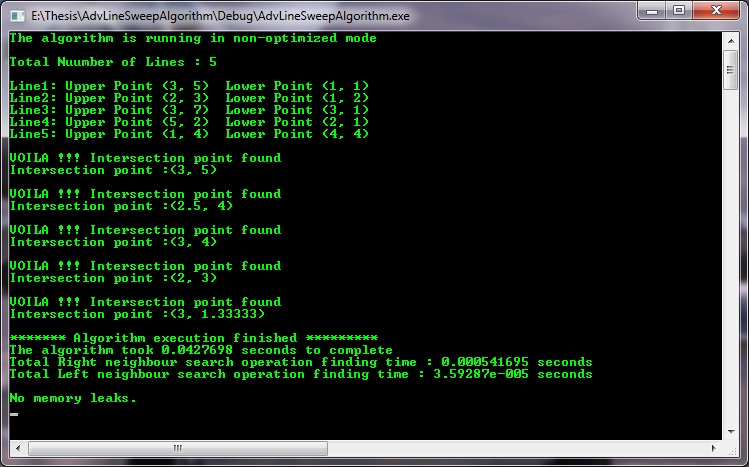
\includegraphics[width=5in, height=3.5in]{Figures/Figure26}}
  \end{center}
  \centering
	\parbox{5in}{\caption{Program output (non-optimized mode).} \label{fig26}} 
\end{figure}
\begin{figure}[ht]
  \begin{center}
   	\fbox{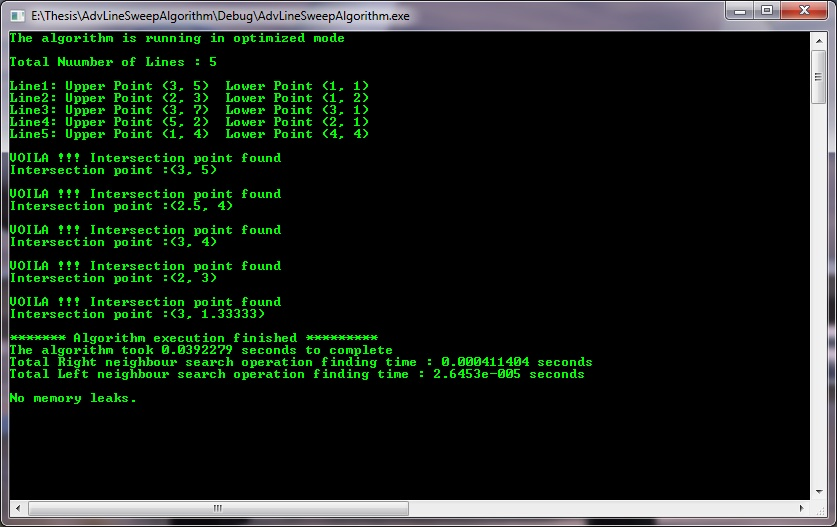
\includegraphics[width=5in, height=3.5in]{Figures/Figure27}}
  \end{center}
  \centering
	\parbox{5in}{\caption{Program output (optimized mode).} \label{fig27}} 
\end{figure}

\clearpage
\section{Results}
Table \ref{tab4} shows the statistical analysis of the neighbor search operation execution time. The program was run on 10 different set of line segments comprising of 5, 50 and 100 set of segments. The line segments were generated using a random number generator program. A generalized random number generator program which is used by the algorithm is provided in Appendix~C.
\begin{table}[hbt]
  \begin{minipage}{6.5in}
	\caption{Statistical Analysis of Neighbor Search Operation on Different Set of Line Segments \label{tab4}}
    \begin{tabular}{||p{1cm}|p{2.5cm}|p{2.5cm}|p{2cm}|p{2cm}|p{2cm}|p{2cm}||}    \hline
       & \multicolumn{2}{|c|}{5 Line Segments} & \multicolumn{2}{|c|}{50 Line Segments} & \multicolumn{2}{|c|}{100 Line Segments} \\ \hline \hline
	   Set & {\it O}(log n) in \newline seconds & {\it O}(1) in \newline seconds & {\it O}(log n) in \newline seconds & {\it O}(1) in \newline seconds & {\it O}(log n) in \newline seconds & {\it O}(1) in \newline seconds \\ \hline
		1 & 0.000585915 & 0.00042009 & 0.0695221 & 0.0584651 & 1.00176 & 0.95164 \\ \hline
		2 & 0.000459967 & 0.000390083 & 0.0536898 & 0.0527888 & 1.19473 & 1.00375 \\ \hline
		3 & 0.000600128 & 0.00055275 & 0.0654452 & 0.0585796 & 1.33972 & 1.11274 \\ \hline
		4 & 0.000571701 & 0.00037508 & 0.0778181 & 0.0547813 & 1.53637 & 1.23689 \\ \hline
		5 & 0.000551170 & 0.000290194 & 0.0508597 & 0.0450012 & 1.64585 & 1.43758 \\ \hline
		6 & 0.000653429 & 0.000301643 & 0.0795048 & 0.0634976 & 1.51176 & 1.38512 \\ \hline
		7 & 0.000414957 & 0.000206491 & 0.0559955 & 0.0466448 & 2.64648 & 2.10963 \\ \hline
		8 & 0.000413378 & 0.000442595 & 0.0591459 & 0.0310854 & 2.10897 & 1.89210 \\ \hline
		9 & 0.000528271 & 0.000338362 & 0.0666241 & 0.0578201 & 1.53587 & 1.31641 \\ \hline
		10 & 0.000595785 & 0.000325333 & 0.0822744 & 0.0631846 & 1.60814 & 1.34926 \\ \hline
    \end{tabular}
  \end{minipage}
\end{table}

\noindent
{\it O}(log n) = Non-optimized (traditional) neighbor search operation time complexity.
\newline \noindent {\it O}(1) = Optimized neighbor search operation time complexity.

\section{Discussion}
Thus it can be clearly seen from Table \ref{tab4} that the optimized mode of the algorithm is definitely better than the non-optimized mode. This difference is short for a small number of input lines but increases gradually as the number of lines increase. For instance we should see a significant improvement in the time complexity of the program, if it is given a huge terra bytes of raster image as an input for solving the map overlay problem (Chapter \ref{chap:intro}) which contains millions of lines. Also it can concluded that the optimized mode of the algorithm increases the neighbor search finding time but it does not contribute much in improving the total running time of the algorithm. This might be because of the way I have coded the algorithm and needs furthur investigation.

% Note that if you want something in single space you can go back and
% forth between single space and normal space by the use of \ssp and
% \nsp.  If you want doublespacing you can use \dsp.  \nsp is normally
% 1.5 spacing unless you use the doublespace option (or savepaper
% option)
%
%(FORMAT) usually you *don't* want to mess with the spacing for your
%(FORMAT) final version.  If you think/know that the thesis template
%(FORMAT) and/or thesis style file is incorrect/incomplete, PLEASE
%(FORMAT) contact the maintainer.  THANK YOU!!!

\chapter{CONCLUSION}
\label{chap:conclusion}
% by labeling the chapter, I can refer to it later using the
% label. (\ref{chap:conclusion}, \pageref{chap:conclusion}) Latex will take care
% of the numbering.

Line Sweep Algorithm is undoubtedly the most popular and widely used algorithm in computational geometry. It can be thought of the essential baby steps required in order to complete the journey of Computational Geometry. Line Sweep algorithm technique is also used in many other computational geometry algorithms like Voronoi diagram and Delaunay triangulation. Proper understanding of the algorithm along with the internal implementation details will definitely be useful for people studying computational geometry algorithms.

I hope that this thesis research will help future students/ researchers in better understanding the algorithm and also provide a working copy of the implementation. Also, this thesis research has introduced the optimized version of the line sweep algorithm which is more efficient that the  traditional algorithm, proved in Chapter \ref{chap:resultsdiscussion}. The traditional algorithm can be replaced by the optimized version achieving the same result, but in a short time. This improvement will be particularly evident for large number of input values where the size of status structure $\tau$ is huge.

Also it can be concluded that using the right tools, methods and technologies to develop a software program can be definitely beneficial. This thesis research has explored the usage of SVN version control software, Visual Studio Integrated Development Environment (IDE) for building C++ programs, power of C++ language features such as operator overloading and templates. Also following good software engineering practices such as unit testing and following appropriate design patterns can help in achieving a better quality product which is easy to maintain. Also last but not the least this thesis research has also taught me the correct way to find, debug and fix memory leaks which is extremely useful in developing any kind of software and not just computational geometry algorithms. Thus this thesis research has taught me a lot of extra useful things besides understanding and improving the line sweep algorithm.

% Note that if you want something in single space you can go back and
% forth between single space and normal space by the use of \ssp and
% \nsp.  If you want doublespacing you can use \dsp.  \nsp is normally
% 1.5 spacing unless you use the doublespace option (or savepaper
% option)
%
%(FORMAT) usually you *don't* want to mess with the spacing for your
%(FORMAT) final version.  If you think/know that the thesis template
%(FORMAT) and/or thesis style file is incorrect/incomplete, PLEASE
%(FORMAT) contact the maintainer.  THANK YOU!!!

\chapter{FUTURE ENHANCEMENTS}
\label{chap:enhancements}
% by labeling the chapter, I can refer to it later using the
% label. (\ref{chap:enhancements}, \pageref{chap:enhancements}) Latex will take care
% of the numbering.

Initially the program does not have any graphical user interface (GUI) and spits out the output on console. The main focus of the thesis was to understand and implement the basic algorithm and also propose an enhancement to the primary data structure used in the algorithm. Providing a GUI for this algorithm is not too difficult if not trivial and the solution for the source code had already been dynamically linked with Microsoft Foundation Classes (MFC) and linked with Microsoft Active Template Library (ATL COM) libraries so that GUI can be easily programmed. In-fact an ActiveX Control would be the perfect solution for the GUI so that future students/ researchers can benefit greatly by understanding the algorithm graphically.

I personally found it very difficult to visualize the way data structures were maintained internally and would have loved to watch it being modified at each step of the algorithm when event points were being handled. The text book \cite{TEXTBOOK1} does fails to explain in detail the implementation details of the AVL tree which is used in the algorithm and especially the implementation of Insert, Update and Delete functions while following the rule that each internal node needs to store the right most child in its left subtree. Also it was difficult to find any implementation details about this on the internet or any paper published in this matter. I think future students would greatly benefit by the documentation I have provided on this matter but it also might be a good idea to show the graphical animated version of the AVL tree being modified as the sweep line handles the event points in the algorithm. Below is a consolidated list of future enhancements which could be done to the thesis program.
\begin{enumerate}
\item Refactor the code according to the recent MVVM (Model-View-View Model) design pattern.
\item Provide a Graphical User Interface (GUI) in ActiveX Control, WPF or Silverlight.
\item Show the actual data structures in real time with animation as they are modified by the algorithm.
\item Provide an SDK (Software Development Kit) so that developers can use the code in their program using the API's (Application Programming Interface). 
\item Write Unit tests for the project.
\item Submit the project to the ``CGAL" (Computational Geometry Algorithms Library) open source community \cite{CGAL} after thorough testing.
\end{enumerate}

% 
% The bibliography page, must be between main body and appendices
% 
% You must have thbib.bib file in the current directory 
% 
\bibliographystyle{siam}
\bibliography{thbib}


% This includes append.tex
\appendices
%
% If you only have one appendix, you should change the above to:
%\appendix
%

\chapter{GLOSSARY AND ACRONYMS}

\begin{itemize}
\item API : ApplicationProgrammingInterface
\item ATL : Active Template Library
\item AVL : G. M. Adelson-Velskii and E. M. Landis
\item BST : Binary Search Tree
\item CAD : Computer Aided Design
\item CADD : Computer Aided Design and Drafting
\item CAM : Computer Aided Manufacturing
\item COM : Component Object Model
\item DLL : Dynamic Link Library
\item DT(P) : Delaunay Triangulation for a set P
\item DWORD : Double Word
\item ESRI : Environmental Systems Research Institute
\item GIS : Geographic Information Science
\item GPS : Global Positioning System
\item GUI : Graphical User Interface
\item IDE : Integrated Development Environment
\item MFC : Microsoft Foundation Classes
\item MSDN : Microsoft Developer Network
\item MVVM : Model-View-View Model
\item RC : Release Candidate
\item SDK : Software Development Kit
\item UI : User Interface
\item WPF : Windows Presentation Foundation
\end{itemize}

\chapter{ALGORITHM PSEUDO CODE}

\noindent
Pseudo code of the implemented algorithm: \newline

\noindent
METHOD Algorithm
    \newline \hspace*{2em}Generate random lines
    \newline \hspace*{2em}Initialize Event Queue Q using the randomly generated lines
    \newline \hspace*{2em}Initialize Status Structure $\tau$;
    \newline \newline \hspace*{2em}CALL FindIntesections with Q and $\tau$
\newline END METHOD

\noindent
\newline METHOD FindIntersections(EventQueue Q, StatusStructure $\tau$)
    \newline \hspace*{2em} Event Point P = Left most leaf in the Event Queue Q;
    \newline \hspace*{2em} WHILE( P != 0 )
        \newline \hspace*{4em} CALL HandleEventPoint with P and $\tau$
        \newline \hspace*{4em} P = Next adjacent right leaf in Event Queue Q;
    \newline \hspace*{2em} END WHILE
\newline END METHOD \newline

\noindent
\newline METHOD HandleEventPoint(EventPoint P, StatusStructure $\tau$)
    \newline \hspace*{2em} arrayU = Set of line segments whose upper end point is P;
    \newline \hspace*{2em} arrayL = Set of line segments whose lower end point is P;
    \newline \hspace*{2em} arrayC = Set of line segments which contains P somewhere in the middle; \newline
    \newline \hspace*{2em} arrayUnion = Unionof arrayU, arrayL and arrayC; \newline
    \newline \hspace*{2em} IF arrayUnion contains more than 1 element
        \newline \hspace*{4em} P is the intersection point and hence  record it;
    \newline \hspace*{2em} END IF \newline
    \newline \hspace*{2em} arrUnionLowerMiddle = Union of arrayL and arrayC;
    \newline \hspace*{2em} FOR EACH element in arrUnionLowerMiddle
        \newline \hspace*{4em} remove element from Status Structure $\tau$;
    \newline \hspace*{2em} arrUnionUpperMiddle = Union of arrayU and arrayC;
    \newline \hspace*{2em} FOR EACH element in arrUnionUpperMiddle
        \newline \hspace*{4em} remove element from Status Structure $\tau$; \newline
    \newline \hspace*{2em} If arrUnionUpperMiddle contains no elements
        \newline \hspace*{4em} LeftNode = Node to the Left of element in Status Structure $\tau$;
        \newline \hspace*{4em} RightNode = Node to the right of element in Status Structure $\tau$; \newline
        \newline \hspace*{4em} CALL FindNewEvent with LeftNode, RightNode and P;
    \newline \hspace*{2em} ELSE IF
        \newline \hspace*{4em} LeftMostSeg = Left Most segment in arrUnionUpperMiddle;
        \newline \hspace*{4em} LeftNeighbor = Left neigbour of LeftMostSeg in $\tau$; \newline
        \newline \hspace*{4em} CALL FindNewEvent with LeftNeighbor, LeftMostSeg and P \newline
        \newline \hspace*{4em} RightMostSeg = Right Most segment in arrUnionUpperMiddle;
        \newline \hspace*{4em} RightNeighbor = Right neighbor of RightMostSeg in $\tau$; \newline
        \newline \hspace*{4em} CALL FindNewEvent with RightMosstSeg, RightNeighbor and P
    \newline \hspace*{2em} END IF
\newline END METHOD \newline

\noindent
\newline METHOD FindNewEvent(leftSeg, rightSeg, P)
    \newline \hspace*{2em} IF leftSeg and rightSeg intersect below the sweep line or on it and to the right of P and intersection point in not yet present in the Event Queue Q
    \newline \hspace*{4em} Intersection Point detected and hence report it;
    \newline \hspace*{2em} END IF
\newline END METHOD \newline

\chapter{RANDOM NUMBER GENERATION CODE}

\noindent /* RAND.C: This program seeds the random-number generator with the time, then displays 10 random integers */ \newline

\noindent \#include $<$stdlib.h$>$ \newline
\noindent \#include $<$stdio.h$>$ \newline
\noindent \#include $<$time.h$>$ \newline

\noindent void main( void ) \newline
\noindent \{
   \newline \hspace*{2em} int i;
   \newline \hspace*{2em} /* Seed the random-number generator with current time so that the numbers
   \newline \hspace*{2em}    will be different every time we run */ \newline
   \newline \hspace*{2em} srand( (unsigned)time( NULL ) );
   \newline \hspace*{2em} /* Display 10 numbers. */
   \newline \hspace*{2em} for( i = 0;   i $<$ 10;i++ )
   \newline \hspace*{4em} printf( ``  \%6d$\backslash$n", rand() );
\newline \noindent \}

\noindent \newline Output \newline
\noindent \newline 60
\noindent \newline 86
\noindent \newline 22
\noindent \newline 69
\noindent \newline 79
\noindent \newline 73
\noindent \newline 10
\noindent \newline 1
\noindent \newline 83
\noindent \newline 33


% 
% Make the library abstract page
% 
%\begin{libraryabstract}
  % This just inserts the the abstract.tex file
%Line sweep algorithm is probably the most popular algorithm in Computational Geometry. The algorithm basically tries to find intersection points among a set of lines in a Cartesian coordinate space.  The algorithm has many real life usages and hence probably is more popular. In this thesis I am presenting two different implementations of the �Line Sweep algorithm�. The two variations of the algorithm are developed using C++ programming language. C++, is the chosen language as it provides a large amount of control over the program but the algorithm can be potentially developed in any choice of programming language. First implementation represents the algorithm as stated in the text book and in the second implementation I am proposing a slight modification. The goal of the alteration would be to enhance the efficiency of this algorithm by modifying one of the data structure used by line-sweep algorithm, namely status structure such as in the line-segment intersection problem, is the objective of this research. The status structure is used to keep track of the segments currently adjacent to one another and the proposed alteration will increase the efficiency of search operations on this structure. I will then be comparing the search operation time required by the two variants of the algorithm to prove the statement.

Modern Design patterns like iterator and factory pattern have been used to develop the algorithm so that it can be easily applied to other use cases with little or no modifications. All the data structures have been self-implemented without dependency on any third party libraries or dynamic link libraries (DLLs). The primary goal of this project besides understanding and implementing the Line sweep algorithm is to suggest some modifications in the original data structure used in this algorithm in order to make it more efficient. Also the secondary goal is to present a working algorithm so that future students/ researchers can better understand the algorithm when they see the internal data structures being updated as the algorithm proceeds, which is very critical in understanding the overall algorithm.

%\end{libraryabstract}

\end{document}
